% !TEX program = pdflatex
\documentclass[journal]{IEEEtran}
\usepackage[utf8]{inputenc}
\usepackage[T1]{fontenc}
\usepackage[turkish,shorthands=:!]{babel}
\usepackage{amsmath,amssymb,bm}
\usepackage{graphicx}
\usepackage{booktabs}
\usepackage{cite}
\usepackage{url}
\usepackage{balance}

\renewcommand{\figurename}{\c{S}ekil}
\renewcommand{\tablename}{TABLO}
\renewcommand{\abstractname}{\"Ozet}
\renewcommand{\IEEEkeywordsname}{Anahtar Kelimeler}
\renewcommand{\refname}{Kaynaklar}
\markboth{}{}

\title{ZERRE (Model H): Ortak-Yol K\i{}r\i{}n\i{}ml\i{} Optoelektronik \.{I}\c{s}lemcinin Dalga-Opti\u{g}i Tasar\i{}m\i{}, Fiziksel Sentezi ve Fizik-Fark\i{}ndal\i{}kl\i{} E\u{g}itimi}

\author{Hamza~Solak%
\thanks{H.~Solak, T\"urkiye'de ba\u{g}\i{}ms\i{}z ara\c{s}t\i{}rmac\i{}d\i{}r (e-posta: eng.hamzasolak@gmail.com; ORCID: 0009-0004-7541-9620).}}

\begin{document}
\maketitle

\begin{abstract}
Programlanabilir optik sinir a\u{g}\i{} i\c{s}lemcileri \c{c}o\u{g}unlukla pahal\i{} uzamsal \i{}\c{s}\i{}k mod\"ulat\"orlerine ve titre\c{s}ime duyarl\i{} \c{c}ift kollu interferometrelere dayan\i{}r. Bu say\i{}sal tasar\i{}m ve dalga-opti\u{g}i sim\"ulasyon \c{c}al\i{}\c{s}mas\i{}, yayg\i{}n monokrom maskeli stereolitografi (mSLA) s\i{}v\i{} kristal ekranlar\i{} temel alan a\c{c}\i{}k kaynakl\i{} ortak-yol optoelektronik ZERRE (Model H) mimarisini sunmaktad\i{}r. \"Ol\c{c}\"ulm\"u\c{s} nematik zay\i{}flama temelinde hacimsel rezervuarlar termal Rayleigh--Gans sa\c{c}\i{}lmas\i{} (15--40 dB/cm) nedeniyle elenmi\c{s}; pasif matrisli ITO s\"ur\"u\c{s}\"un\"un ise Alt--Pleshko s\i{}n\i{}r\i{} uyar\i{}nca 16 sat\i{}rda kullan\i{}labilir E7 faz aral\i{}\u{g}\i{}n\i{} 4,86 rad'dan (1,00--5,00 V) 0,921 rad'a daraltt\i{}\u{g}\i{} g\"osterilmi\c{s}tir. Skaler A\c{c}\i{}sal Spektrum yay\i{}l\i{}m\i{} ve kuple Jones mod\"ulasyonu i\c{c}in t\"uretilen kapal\i{} form Wirtinger e\c{s}lenik operat\"or\"u (sonlu farklarla ba\u{g}\i{}l hata $5{,}52\times 10^{-7}$), modellenmemi\c{s} donan\i{}m kusurlar\i{}na kar\c{s}\i{} Fizik-Fark\i{}ndal\i{}kl\i{} E\u{g}itimi (PAT) m\"umk\"un k\i{}lar. \"U\c{c} tohumda ($N_{\mathrm{test}}=1000$) t\"um okuma kafalar\i{}n\i{}n ayn\i{} \c{c}apraz-entropi/Adam protokol\"uyle e\c{s}lendi\u{g}i k\i{}s\i{}tl\i{} $8\times 8$ dedekt\"or rejiminde PAT, lineer MNIST do\u{g}rulu\u{g}unu e\c{s}le\c{s}mi\c{s} rastgele opti\u{g}e g\"ore \%71,07'den \%78,40'a (+7,33 puan) \c{c}\i{}kar\i{}rken do\u{g}rudan dijital alan havuzlaman\i{}n (\%87,00) 8,60 puan gerisinde kal\i{}r. Tam $32\times 32$ okuma ve hibrit \c{c}ok katmanl\i{} alg\i{}lay\i{}c\i{}yla nominal-ikiz \"ust s\i{}n\i{}r\i{} MNIST'te \%94,67 ve Fashion-MNIST'te \%84,43'e ula\c{s}\i{}rken (kusurlu sistem: \%91,07, \%81,47), bu de\u{g}erler ham piksel (\%93,93, \%85,17) ve rastgele optik (\%94,20, \%84,70) MLP'leriyle e\c{s}de\u{g}erdir. 15 dalga boyu Zernike sapmas\i{}nda k\"or PAT \%77,30'a ula\c{s}\i{}r (yaln\i{}z-kafa \%76,67; +0,63 puan birle\c{s}ik SS i\c{c}inde) ve 4-bit basamaklamada \%94,8'i korur; ancak pert\"urbe LC e\u{g}risi, kamera gammas\i{} ve benek i\c{c}eren yap\i{}sal uyumsuzlukta yaln\i{}z-kafa kalibrasyonunun gerisinde kal\i{}r (\%76,80 ve \%79,13). Tahmini bile\c{s}en b\"ut\c{c}esi 784--959 USD'dir.
\end{abstract}

\begin{IEEEkeywords}
A\c{c}\i{}sal spektrum y\"ontemi, k\i{}r\i{}n\i{}ml\i{} sinir a\u{g}lar\i{}, s\i{}v\i{} kristal mod\"ulat\"orler, optoelektronik hesaplama, fizik-fark\i{}ndal\i{}kl\i{} e\u{g}itim, Wirtinger e\c{s}lenik.
\end{IEEEkeywords}

% ============================================================================
\section{Giri\c{s}}
% ============================================================================

Modern CMOS ve GPU h\i{}zland\i{}r\i{}c\i{}lar\i{}nda toplam \c{c}\i{}kar\i{}m enerjisinin \%60 ila \%90'\i{}, aritmetik i\c{s}lemlerden \c{c}ok a\u{g}\i{}rl\i{}klar\i{}n ve aktivasyonlar\i{}n bellek hiyerar\c{s}isi ile ara ba\u{g}lant\i{}lar boyunca ta\c{s}\i{}nmas\i{}nda harcanmaktad\i{}r \cite{horowitz2014computing,sze2017efficient}. Serbest uzay ve entegre optik hesaplama mimarileri bu veri ta\c{s}\i{}ma darbo\u{g}az\i{}n\i{} analog d\"uzeyde ele al\i{}r: yap\i{}land\i{}r\i{}lm\i{}\c{s} k\i{}r\i{}n\i{}ml\i{} veya faz mod\"ulasyonlu bir ortamdan ge\c{c}en \i{}\c{s}\i{}k alan\i{}, $10\,\text{cm}$ uzunlu\u{g}undaki bir optik yoldan $\sim 0{,}33\,\text{ns}$ s\"urede ge\c{c}erken uzamsal s\"uperpozisyon yoluyla yo\u{g}un do\u{g}rusal d\"on\"u\c{s}\"umleri pasif bi\c{c}imde icra eder \cite{wetzstein2020inference,psaltis1985optical,lin2018alloptical}.

3B bask\i{}l\i{} k\i{}r\i{}n\i{}ml\i{} derin sinir a\u{g}lar\i{} ($\text{D}^2\text{NN}$) terahertz band\i{}nda pasif s\i{}n\i{}fland\i{}rma ortaya koymu\c{s} \cite{lin2018alloptical}, ancak sabit dielektrik plakalar\i{}n g\"orev de\u{g}i\c{s}imine uyarlanamamas\i{} nedeniyle ara\c{s}t\i{}rmalar yeniden yap\i{}land\i{}r\i{}labilir sistemlere y\"onelmi\c{s}tir. Takip eden \c{c}al\i{}\c{s}malarda nanofotonik Mach--Zehnder a\u{g}lar\i{} \cite{shen2017deep}, b\"uy\"uk \"ol\c{c}ekli k\i{}r\i{}n\i{}ml\i{} i\c{s}leme birimleri \cite{zhou2021largescale}, entegre fotonik tens\"or \c{c}ekirdekleri \cite{feldmann2021parallel}, zaman-dalga boyu \c{c}o\u{g}ullamas\i{} \cite{xu2021tops} ve hibrit optik-elektronik evri\c{s}imli \"on u\c{c}lar \cite{chang2018hybrid} geli\c{s}tirilmi\c{s}tir. Cep tipi s\i{}v\i{} kristal televizyonlarla ba\c{s}layan \cite{yu1990lctv} ve g\"uncel uzamsal matris \c{c}arp\i{}c\i{}larla \cite{spall2020reconfigurable} s\"urd\"ur\"ulen paralel \c{c}al\i{}\c{s}malar da ticari ekranlar\i{}n programlanabilir optik a\u{g}\i{}rl\i{}k olarak kullan\i{}labilece\u{g}ini g\"ostermi\c{s}tir.

Buna kar\c{s}\i{}n deneysel eri\c{s}ilebilirli\u{g}i k\i{}s\i{}tlayan \"u\c{c} m\"uhendislik engeli s\"urmektedir: laboratuvar tipi LCOS mod\"ulat\"orler d\"uzlem ba\c{s}\i{}na 8.000--40.000~USD maliyet gerektirmekte; \c{c}ift kollu interferometreler nanometre \"ol\c{c}e\u{g}indeki yol kaymalar\i{}nda ($\lambda/4 \approx 133\,\text{nm}$) s\"on\"umlenmeye u\u{g}ramakta \cite{shen2017deep}; ideal say\i{}sal modellerde e\u{g}itilen a\u{g}\i{}rl\i{}klar ise fiziksel hiza hatalar\i{} ve pasif matrisli s\i{}v\i{} kristal h\"ucrelerdeki etkin (RMS) voltaj kenetlenmesi nedeniyle do\u{g}ruluk kaybetmektedir.

Bu makale, \textbf{ZERRE (Model H)} ortak-yol optoelektronik i\c{s}lemci mimarisi ile a\c{c}\i{}k kaynakl\i{} dalga-opti\u{g}i say\i{}sal ikizinin tasar\i{}m\i{}n\i{} ve sim\"ulasyon analizini sunmaktad\i{}r; bu a\c{s}amada hen\"uz fiziksel bir masa\"ust\"u prototip kurulmam\i{}\c{s} ve optik \"ol\c{c}\"um al\i{}nmam\i{}\c{s}t\i{}r. Nematik s\i{}v\i{} kristallerdeki hacimsel sa\c{c}\i{}lma s\i{}n\i{}rlar\i{}ndan \cite{wu1987scattering} yola \c{c}\i{}k\i{}larak sekiz aday topoloji (Model~A--H) taranm\i{}\c{s} ve birimi 40--60~USD olan monokrom mSLA 2K ekranlara dayal\i{} d\"uzlemsel $7\,\mu\text{m}$ ince h\"ucre mimarisi se\c{c}ilmi\c{s}tir. Alt--Pleshko teoremi \cite{alt1974scanning} uygulanarak $16\times 16$ pasif matris taramas\i{}n\i{}n ($1/5$ gerilim \"ongerilimi) RMS se\c{c}im oran\i{}n\i{} $1{,}290994$'e k\i{}s\i{}tlad\i{}\u{g}\i{} ve kullan\i{}labilir E7 faz aral\i{}\u{g}\i{}n\i{} $5{,}28\times$ daraltarak $4{,}86\,\text{rad}$'dan $0{,}921\,\text{rad}$'a d\"u\c{s}\"urd\"u\u{g}\"u g\"osterilmi\c{s}tir. Son olarak, A\c{c}\i{}sal Spektrum yay\i{}l\i{}m\i{} \"uzerinden kapal\i{} form Wirtinger e\c{s}lenik gradyan\i{} t\"uretilerek kusurlu fiziksel sistem sim\"ulat\"or\"u \"uzerinde Fizik-Fark\i{}ndal\i{}kl\i{} E\u{g}itim (PAT) \cite{wright2022pat,hughes2018insitu} uygulanm\i{}\c{s}; \"u\c{c} rastgele tohumda MNIST ve Fashion-MNIST ba\c{s}ar\i{}m\i{} mekanik, termal, ortam \i{}\c{s}\i{}\u{g}\i{}, bit kuantizasyonu, alt-a\c{c}\i{}kl\i{}k dolulu\u{g}u ve Zernike sapma testleriyle birlikte say\i{}sal olarak de\u{g}erlendirilmi\c{s}tir.

\begin{figure*}[!t]
  \centering
  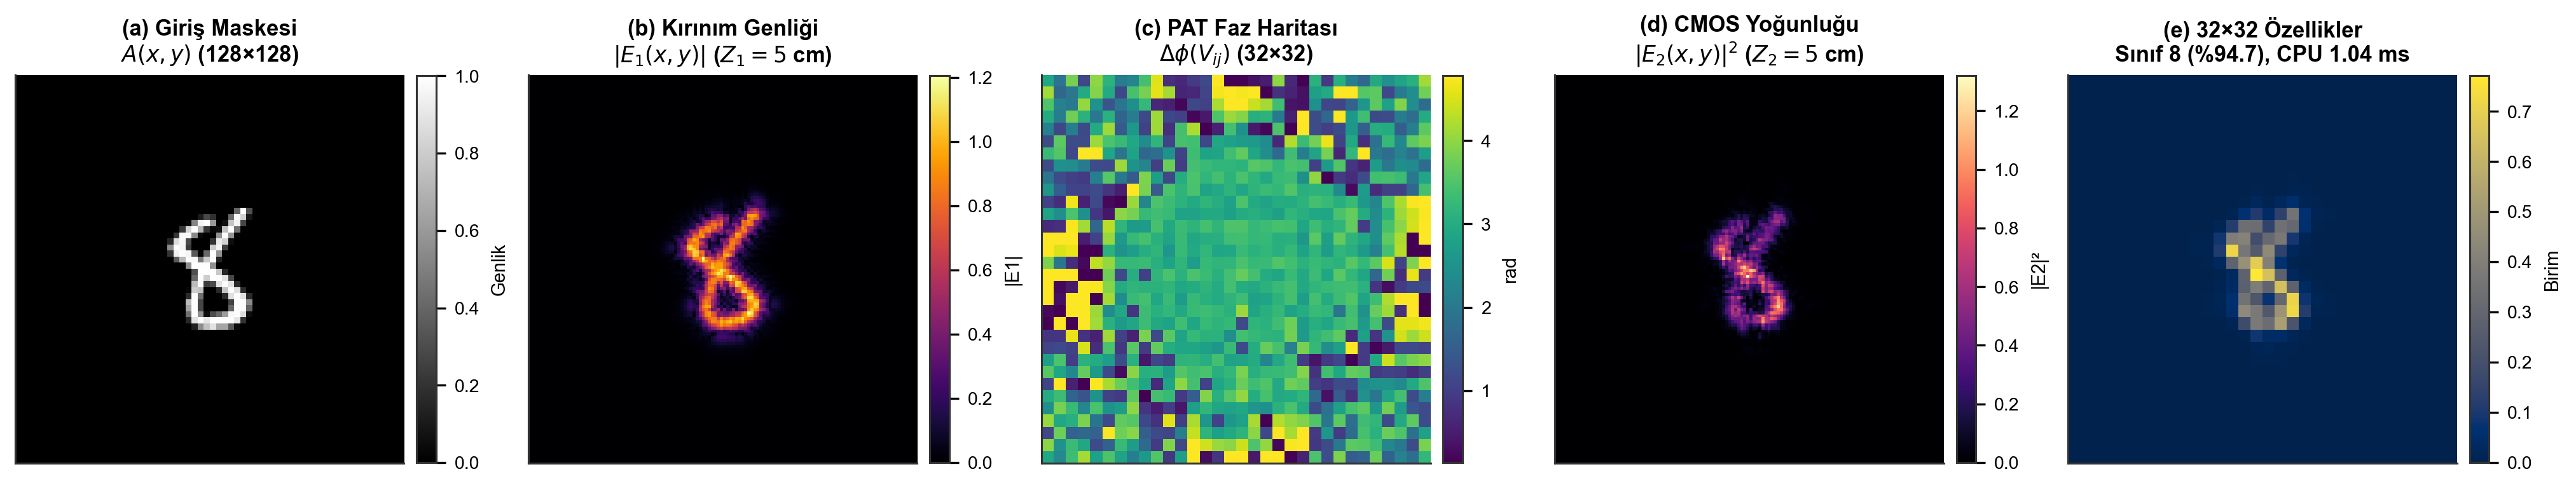
\includegraphics[width=\textwidth]{figures/makale_fig1_dalga_tr.png}
  \caption{ZERRE Model H dalga-opti\u{g}i hatt\i{}nda el yaz\i{}s\i{} bir MNIST rakam\i{}n\i{}n (``8'') skaler ileri yay\i{}l\i{}m\i{} ($N=128^2$, $\Delta x=47\,\mu\text{m}$): \textbf{(a)}~monokrom mSLA panelde kodlanan $A(x,y)$ genlik maskesi; \textbf{(b)}~$Z_1=5\,\text{cm}$ A\c{c}\i{}sal Spektrum yay\i{}l\i{}m\i{} sonras\i{} LC a\u{g}\i{}rl\i{}k d\"uzlemindeki k\i{}r\i{}n\i{}m genli\u{g}i $|E_1(x,y)|$; \textbf{(c)}~PAT ile e\u{g}itilmi\c{s} $32\times 32$ aktif LC faz haritas\i{} $\Delta\phi(V_{ij})$ [rad]; \textbf{(d)}~\c{c}apraz analiz\"or ve $Z_2=5\,\text{cm}$ sonras\i{} CMOS sens\"or yo\u{g}unlu\u{g}u $|E_2(x,y)|^2$; \textbf{(e)}~$32\times 32$ havuzlanm\i{}\c{s} optik \"ozellik haritas\i{} (\%94,7 g\"uvenle S\i{}n\i{}f~8 tahmini; $N=128^2$ \i{}zgarada ortanca CPU sim\"ulasyon s\"uresi $1{,}04\,\text{ms}$).}
  \label{fig:wave_chain}
\end{figure*}

% ============================================================================
\section{Mimari Sentez ve Fiziksel K\i{}s\i{}tlar}
% ============================================================================

\subsection{Hacimsel Nematik Sa\c{c}\i{}lma S\i{}n\i{}r\i{}: K\"ureye Kar\c{s}\i{} \.{I}nce H\"ucre}
De\u{g}erlendirilen sekiz kavramsal topolojiden (Model~A--H) d\"ort hacimsel nematik rezervuar tasar\i{}m\i{} (32 elektrotlu Fibonacci k\"uresi Model~A, yar\i{}-k\"ure hibrit kase Model~C, fotodiyot adreslemeli k\"ure Model~F ve k\"uresel ITO matrisi Model~G), \"u\c{c} boyutlu optik kar\i{}\c{s}\i{}m sa\u{g}lamak \"uzere santimetre \"ol\c{c}ekli borosilikat kaplar\i{} ($\varnothing 100\,\text{mm}$) Merck E7 ile doldurmay\i{} incelemi\c{s}tir. Ancak nematik fazda termal direkt\"or dalgalanmalar\i{}, g\"or\"un\"ur dalga boylar\i{}nda i\c{c}sel so\u{g}urmadan yakla\c{s}\i{}k iki mertebe daha g\"u\c{c}l\"u Rayleigh--Gans sa\c{c}\i{}lmas\i{} \"ureterek $\alpha_{\mathrm{scat}} \approx 15\text{--}40\,\text{dB/cm}$ zay\i{}flama olu\c{s}turur \cite{wu1987scattering}. $L = 10\,\text{cm}$ optik yol boyunca balistik iletim kayb\i{} $150\text{--}400\,\text{dB}$ d\"uzeyine ula\c{s}\i{}r; koherent dalga cephesi foton dif\"uzyonuna d\"on\"u\c{s}\"ur ve mekanik sars\i{}nt\i{} alt\i{}nda s\i{}v\i{} \c{c}alkalanmas\i{} direkt\"or alan\i{}n\i{} bozar.

Buna kar\c{s}\i{}l\i{}k E7 katman\i{}n\i{} $d \le 7\,\mu\text{m}$ d\"uzlemsel bir bo\c{s}lu\u{g}a hapsetmek sa\c{c}\i{}lma kayb\i{}n\i{} $0{,}003\text{--}0{,}03\,\text{dB}$ aral\i{}\u{g}\i{}na indirir ve k\i{}lcal kuvvetler s\i{}v\i{}y\i{} sabitler. $\lambda = 532\,\text{nm}$ i\c{c}in $7\,\mu\text{m}$ saf E7 ($\Delta n = 0{,}225$) $18{,}60\,\text{rad}$ ($\approx 5{,}92\pi$) \c{c}ok-mertebeli faz gecikmesi \"uretirken, tek-mertebeli \c{c}al\i{}\c{s}ma penceresi
\begin{equation}
  \Delta\phi_{\max} = \frac{2\pi}{\lambda}\,\Delta n_{\mathrm{eff}}\, d \approx 4{,}97\,\text{rad} \; (\approx 1{,}58\pi)
  \label{eq:max_phase}
\end{equation}
ya ticari mSLA TFT panellerdeki florlu nematik kar\i{}\c{s}\i{}mlarla ($\Delta n_{\mathrm{eff}} \approx 0{,}060$, $d = 7\,\mu\text{m}$), ya $d = 1{,}87\,\mu\text{m}$ ince E7 h\"ucreyle, ya da $7\,\mu\text{m}$ E7'nin $V \ge 2{,}2\,\text{V}$ RMS \"ongerilim penceresinde sa\u{g}lan\i{}r. Kalan d\"uzlemsel ince h\"ucre adaylar\i{} aras\i{}nda pasif $16\times 16$ ITO plaka (Model~B) B\"ol\"um~II-C'de incelenen \c{c}o\u{g}ullama s\i{}n\i{}r\i{}na tak\i{}lmakta, tek 7 katmanl\i{} y\i{}\u{g}\i{}n (Model~D) $7\,\mu\text{m}$ h\"ucre kesitini belirlemekte ve 3 katmanl\i{} kaskad y\i{}\u{g}\i{}n (Model~E) iletim kayb\i{} ile hizalama maliyetini katlamakta; b\"oylece tek a\u{g}\i{}rl\i{}k d\"uzlemli ortak-yol mimari (Model~H) uygulanabilir temel sentez olarak \"one \c{c}\i{}kmaktad\i{}r. Kal\i{}n h\"ucre sa\c{c}\i{}lmas\i{}na y\"onelik olas\i{} deneyler ise k\"ure imalat\i{} \"oncesinde d\"u\c{s}\"uk maliyetli $1\,\text{cm}$ cam k\"uvette yap\i{}lacak ge\c{c}irgenlik testiyle s\i{}n\i{}rland\i{}r\i{}lm\i{}\c{s}t\i{}r.

\subsection{Giri\c{s} Kodlama: Ticari mSLA Monokrom LCD Paneller}
Maskeli stereolitografi (mSLA) 3B yaz\i{}c\i{}lar i\c{c}in seri \"uretilen monokrom LCD paneller, ara\c{s}t\i{}rma s\i{}n\i{}f\i{} LCOS mod\"ulat\"orlere eri\c{s}ilebilir bir se\c{c}enek olu\c{s}turur. Yayg\i{}n $5{,}5\,\text{in\c{c}}$ paneller $1440\times 2560$ piksel ($\sim 47\,\mu\text{m}$ ad\i{}m; $\sim 6{,}1\,\text{in\c{c}}$ modellerde $1620\times 2560$) sunar, RGB renk filtresi ve arka ayd\i{}nlatma i\c{c}ermeden \c{c}\i{}plak transmisif vana olarak gelir ve standart HDMI--MIPI s\"ur\"uc\"u kart\i{}yla $60\,\text{Hz}$ 8-bit gri tonda 40--60~USD kar\c{s}\i{}l\i{}\u{g}\i{}nda temin edilir. TFT veri yollar\i{} net a\c{c}\i{}kl\i{}k ge\c{c}irgenli\u{g}ini \%4--\%8 d\"uzeyine d\"u\c{s}\"urse de $100\,\text{mW}$ $532\,\text{nm}$ DPSS lazer ve milisaniye mertebesinde CMOS pozlamas\i{} bunu telafi eder; $16{,}7\,\text{ms}$ \c{c}er\c{c}eve yenileme s\"uresi de E7'nin $\sim 50\,\text{ms}$ viskoelastik gev\c{s}eme s\"uresinden h\i{}zl\i{}d\i{}r.

\begin{figure*}[!t]
  \centering
  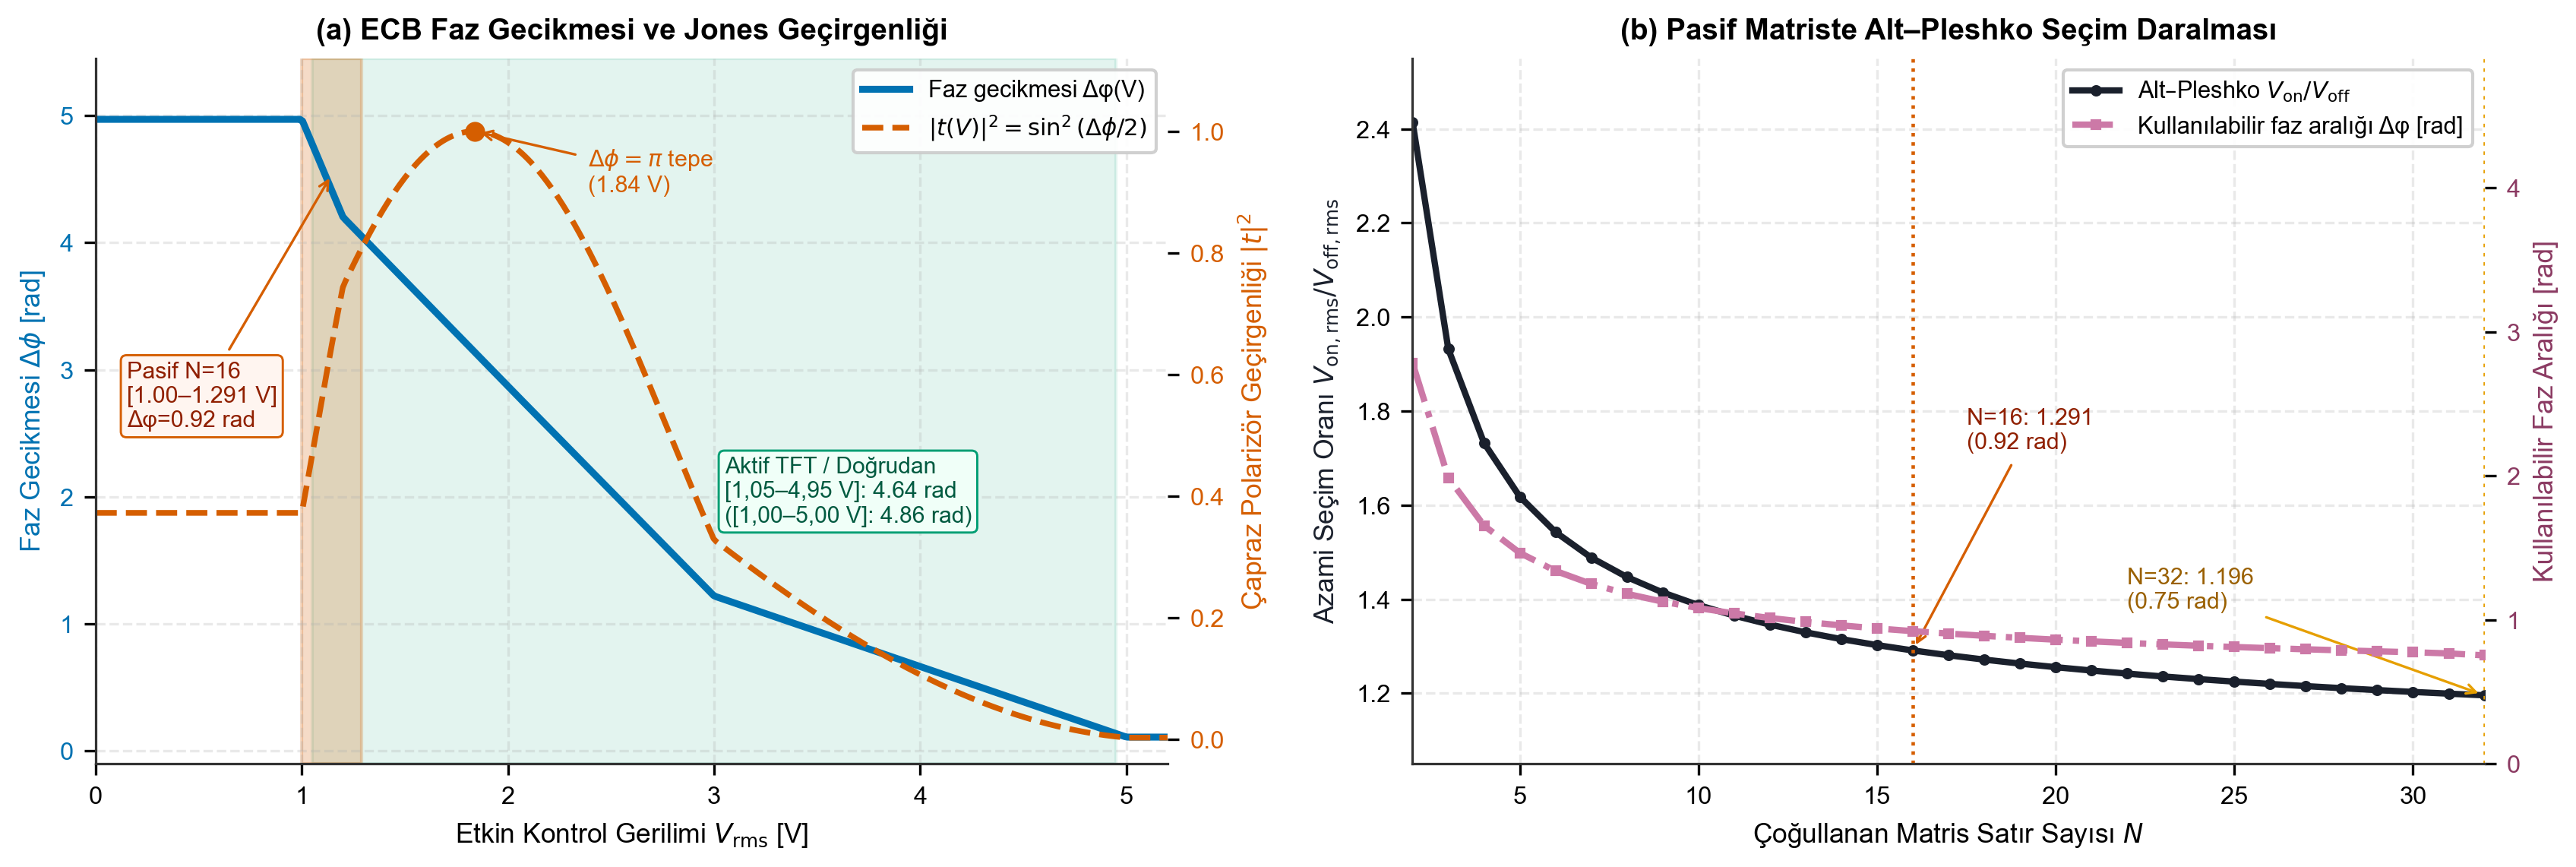
\includegraphics[width=0.96\textwidth]{figures/makale_fig2_alt_pleshko_tr.png}
  \caption{Nematik s\i{}v\i{} kristal a\u{g}\i{}rl\i{}k katman\i{}nda pasif matris \c{c}o\u{g}ullama s\i{}n\i{}r\i{}: \textbf{(a)}~ECB faz gecikmesi $\Delta\phi(V_{\mathrm{rms}})$ (mavi, sol eksen) ve $1{,}84\,\text{V}$ civar\i{}nda $\Delta\phi = \pi$ noktas\i{}nda tepe yapan monoton olmayan \c{c}apraz polariz\"or yo\u{g}unluk ge\c{c}irgenli\u{g}i $|t(V)|^2 = \sin^2(\Delta\phi/2)$ (kesikli turuncu, sa\u{g} eksen). K\i{}rm\i{}z\i{} alan $16\times 16$ pasif taraman\i{}n dayatt\i{}\u{g}\i{} $[1{,}00\,\text{V}, 1{,}291\,\text{V}]$ ($0{,}921\,\text{rad}$) penceresini, ye\c{s}il alan ise $[1{,}05, 4{,}95]\,\text{V}$ aktif PAT penceresindeki $4{,}64\,\text{rad}$ aral\i{}\u{g}\i{}n\i{} ($[1{,}00, 5{,}00]\,\text{V}$ \"uzerinde $4{,}86\,\text{rad}$) g\"osterir. \textbf{(b)}~Sat\i{}r say\i{}s\i{} $N$ $2$'den $32$'ye \c{c}\i{}karken Alt--Pleshko se\c{c}im oran\i{}n\i{}n ve faz aral\i{}\u{g}\i{}n\i{}n d\"u\c{s}\"u\c{s}\"u.}
  \label{fig:alt_pleshko}
\end{figure*}

\subsection{Pasif Matris S\"ur\"u\c{s}te Alt--Pleshko RMS K\i{}s\i{}t\i{}}
$N\times N$ elektrotlu bir \"org\"uy\"u $2N$ sat\i{}r/s\"utun kanal\i{}yla zaman \c{c}o\u{g}ullamal\i{} (\"orne\u{g}in $N=16$ i\c{c}in $1/5$ gerilim \"ongerilimi) s\"urmek ilk bak\i{}\c{s}ta ekonomik g\"or\"un\"ur. Ancak nematik s\i{}v\i{} kristallerdeki dielektrik tork elektrik alan\i{}n karesiyle ($\propto E^2$) orant\i{}l\i{} oldu\u{g}undan ve $\sim 50\,\text{ms}$ pencere \"uzerinden ortaland\i{}\u{g}\i{}ndan, her h\"ucre anl\i{}k darbeler yerine t\"um tarama periyodu boyunca olu\c{s}an etkin (RMS) gerilime yan\i{}t verir:
\begin{equation}
  V_{\mathrm{rms}}(i,j) = \sqrt{\frac{1}{N}\left(V_{\mathrm{sel}} + U_{ij}V_{\mathrm{data}}\right)^2 + \frac{1}{N}\sum_{r\neq i}\left(U_{rj}V_{\mathrm{data}}\right)^2},
  \label{eq:vrms}
\end{equation}
burada $U_{rj}\in[-1, +1]$ normalize s\"utun a\u{g}\i{}rl\i{}klar\i{}d\i{}r. Optimum $V_{\mathrm{sel}}/V_{\mathrm{data}} = \sqrt{N}$ ($N=16$ i\c{c}in $4$) oran\i{}nda Alt--Pleshko teoremi \cite{alt1974scanning} ula\c{s}\i{}labilir en y\"uksek se\c{c}im oran\i{}n\i{}
\begin{equation}
  \frac{V_{\mathrm{on,rms}}}{V_{\mathrm{off,rms}}} \le \sqrt{\frac{\sqrt{N}+1}{\sqrt{N}-1}}
  \label{eq:alt_pleshko}
\end{equation}
ile s\i{}n\i{}rlar. $N=16$ sat\i{}r i\c{c}in bu s\i{}n\i{}r $\sqrt{5/3} \approx 1{,}290994$'t\"ur ($N=32$ i\c{c}in $1{,}195606$'ya d\"u\c{s}er). Se\c{c}ilmemi\c{s} pikseller $1{,}00\,\text{V}$ Freedericksz e\c{s}i\u{g}inde tutuldu\u{g}unda se\c{c}ili piksel en fazla $1{,}291\,\text{V}$ RMS alabilir; b\"oylece E7 faz mod\"ulasyon aral\i{}\u{g}\i{} $4{,}86\,\text{rad}$'dan $0{,}921\,\text{rad}$'a ($5{,}28\times$ daralma, \c{S}ekil~\ref{fig:alt_pleshko}a) inerken \eqref{eq:vrms}'deki toplam terimi s\"utun boyunca \c{c}apraz etkile\c{s}im olu\c{s}turur. Bu nedenle Model H, pasif tarama yerine do\u{g}rudan AC kuplajl\i{} PWM kanallar\i{}n\i{} veya her pikselinde depolama kondansat\"or\"u bar\i{}nd\i{}ran ikinci bir aktif-matris TFT mSLA panelini benimser.

% ============================================================================
\section{Dalga-Opti\u{g}i Modeli ve Fizik-Fark\i{}ndal\i{}kl\i{} E\u{g}itim}
% ============================================================================

\subsection{A\c{c}\i{}sal Spektrum Yay\i{}l\i{}m\i{} ve Kuple Jones Mod\"ulasyonu}
Giri\c{s} mSLA paneli taraf\i{}ndan genlik mod\"ulasyonuna u\u{g}rat\i{}lan do\u{g}rusal polarize ($0^\circ$) $532\,\text{nm}$ d\"uzlem dalga $E_0(x,y) = A(x,y)$ alan\i{}n\i{} olu\c{s}turur ve $Z_1 = 5\,\text{cm}$ serbest uzay boyunca paraksiyel olmayan skaler A\c{c}\i{}sal Spektrum Y\"ontemi (ASM) ile yay\i{}l\i{}r \cite{goodman2017fourier}:
\begin{align}
  E_1 &= \mathcal{P}_{Z_1}\{E_0\} = \mathcal{F}^{-1}\!\left\{\mathcal{F}\{E_0\} \odot H(f_x, f_y; Z_1)\right\}, \label{eq:asm} \\
  H(f_x, f_y; z) &= \exp\!\left(i\frac{2\pi}{\lambda}z\sqrt{1 - \lambda^2 f_x^2 - \lambda^2 f_y^2}\right) \cdot \mathbb{I}_{f_x^2+f_y^2 < \lambda^{-2}}, \label{eq:transfer}
\end{align}
burada s\"on\"uml\"u bile\c{s}enler filtrelenir. A\u{g}\i{}rl\i{}k d\"uzleminde analitik model, \c{c}apraz polariz\"orler ($0^\circ/90^\circ$) aras\i{}nda $45^\circ$ y\"onlendirilmi\c{s} paralel-hizal\i{} elektriksel kontroll\"u \c{c}ift-k\i{}r\i{}l\i{}m (ECB) h\"ucresi varsayar; k\"uresel sabit faz haricinde skaler Jones ge\c{c}i\c{s}i
\begin{equation}
  t(V_{ij}) = \sin\!\left(\frac{\Delta\phi(V_{ij})}{2}\right) \exp\!\left(i\frac{\Delta\phi(V_{ij})}{2}\right)
  \label{eq:jones}
\end{equation}
olup $Z_2 = 5\,\text{cm}$ yay\i{}l\i{}m\i{} sonras\i{} $I_{\mathrm{CMOS}} = |\mathcal{P}_{Z_2}\{E_1 \odot M(\mathbf{V})\}|^2$ yo\u{g}unlu\u{g}u ortalanm\i{}\c{s} $K\times K$ dedekt\"or bloklar\i{}nda havuzlanarak $\mathbf{f} \in \mathbb{R}^{K^2}$ vekt\"or\"une d\"on\"u\c{s}t\"ur\"ul\"ur (\c{S}ekil~\ref{fig:wave_chain}). Par\c{c}al\i{}-do\u{g}rusal elektro-optik e\u{g}ride gerilim artt\i{}k\c{c}a $\Delta\phi(V)$ monoton bi\c{c}imde $4{,}97\,\text{rad}$'dan ($1{,}00\,\text{V}$) $0{,}11\,\text{rad}$'a ($5{,}00\,\text{V}$) inerken ($4{,}86\,\text{rad}$ toplam aral\i{}k; aktif PAT eniyileme s\i{}n\i{}rlar\i{} $[1{,}05, 4{,}95]\,\text{V}$ i\c{c}inde $4{,}64\,\text{rad}$), $|t(V)|^2 = \sin^2(\Delta\phi/2)$ \c{c}arpan\i{} monoton de\u{g}ildir ve $\Delta\phi = \pi$ noktas\i{}nda tepe yapar (\c{S}ekil~\ref{fig:alt_pleshko}a). Denklem~\eqref{eq:jones} ticari b\"uk\"uml\"u nematik (TN) mSLA paneller i\c{c}in kapal\i{} formda kuple genlik--faz vekili g\"orevi g\"or\"ur \cite{lu1990lctv}; TN panelle fiziksel kurulumda polariz\"or a\c{c}\i{}lar\i{}n\i{}n yeniden hizalanmas\i{} ve deneysel kalibrasyon gerekir. PAT ileri/e\c{s}lenik FFT yay\i{}l\i{}mlar\i{} \texttt{complex64} duyarl\i{}kta, PAT-d\i{}\c{s}\i{} analitik taramalar ve de\u{g}erlendirme yollar\i{} ise \texttt{complex128} duyarl\i{}kta y\"ur\"ut\"ul\"ur.

Piksel ad\i{}m\i{} $\Delta x = 47\,\mu\text{m}$ iken kritik ASM \"ornekleme boyutu $N_{\mathrm{crit}} = \lambda Z_1 / \Delta x^2 \approx 12{,}0$ pikseldir; dolay\i{}s\i{}yla $N=128$ (ve $256$) \i{}zgaralar\i{} Nyquist ko\c{s}ulunu on kattan fazla a\c{s}ar. $Z_1$ boyunca azami k\i{}r\i{}n\i{}m yay\i{}lmas\i{} $Z_1\lambda/(2\Delta x) = 0{,}283\,\text{mm}$ olup $N=128$'deki $1{,}69\,\text{mm}$ ($2{,}63\,\text{mm}$ giri\c{s} g\"or\"unt\"us\"u) ve $0{,}75\,\text{mm}$ ($4{,}51\,\text{mm}$ aktif h\"ucre) s\i{}f\i{}r-dolgulu koruma bantlar\i{}n\i{}n ($N=256$'da $2{,}73\,\text{mm}$ ve $1{,}50\,\text{mm}$) i\c{c}inde kalarak dairesel sarmay\i{} bast\i{}r\i{}r.

\subsection{Wirtinger Kalk\"ul\"us\"u ile Analitik E\c{s}lenik Geri Yay\i{}l\i{}m}
Y\"uzlerce elektrot i\c{c}in sonlu fark de\u{g}erlendirmesi yapmadan skaler kay\i{}p $\mathcal{L}$'nin $\mathbf{V}$ gerilimlerine g\"ore t\"urevini almak \"uzere, $I = E_2 E_2^*$ i\c{c}in sens\"or d\"uzlemindeki karma\c{s}\i{}k Wirtinger hata alan\i{}
\begin{equation}
  G_{\mathrm{cam}} = 2 \left(\frac{\partial \mathcal{L}}{\partial I}\right) \odot E_2
  \label{eq:wirtinger}
\end{equation}
bi\c{c}iminde yaz\i{}l\i{}r. Ayr\i{}k ger\c{c}el i\c{c} \c{c}arp\i{}m $\langle u, v \rangle = \operatorname{Re}\sum u^* v$ alt\i{}nda ASM operat\"or\"un\"un Hermitik e\c{s}leni\u{g}i $-Z_2$ y\"on\"unde geri yay\i{}l\i{}md\i{}r:
\begin{equation}
  G_{\mathrm{mask}} = \mathcal{P}_{Z_2}^{\dagger}\{G_{\mathrm{cam}}\} = \mathcal{F}^{-1}\!\left\{\mathcal{F}\{G_{\mathrm{cam}}\} \odot H^*(f_x, f_y; Z_2)\right\}.
  \label{eq:adjoint}
\end{equation}
Her elektrot makro-pikseli $\Omega_{ij}$ \"uzerinden $G_{t,ij} = \sum_{(u,v)\in\Omega_{ij}} E_1^*(u,v) G_{\mathrm{mask}}(u,v)$ toplan\i{}p $dt/d\phi = \frac{1}{2}e^{i\phi}$ uyguland\i{}\u{g}\i{}nda tek bir ters/ileri FFT \c{c}iftiyle tam voltaj gradyan\i{} elde edilir:
\begin{equation}
  \frac{\partial \mathcal{L}}{\partial V_{ij}} = \operatorname{Re}\!\left\{G_{t,ij}^* \cdot \frac{1}{2}e^{i\Delta\phi(V_{ij})}\right\} \cdot \left.\frac{d\Delta\phi}{dV}\right|_{V_{ij}}.
  \label{eq:grad_v}
\end{equation}
Merkezi sonlu farklarla ($\varepsilon = 10^{-6}$) yap\i{}lan do\u{g}rulamada \eqref{eq:grad_v}, aktif modda $5{,}52 \times 10^{-7}$, pasif Alt--Pleshko zincir kural\i{} alt\i{}nda ise $7{,}46 \times 10^{-7}$ ba\u{g}\i{}l $L_2$ hatas\i{} vermektedir (\c{S}ekil~\ref{fig:ablation_pat}b).

\begin{figure*}[!t]
  \centering
  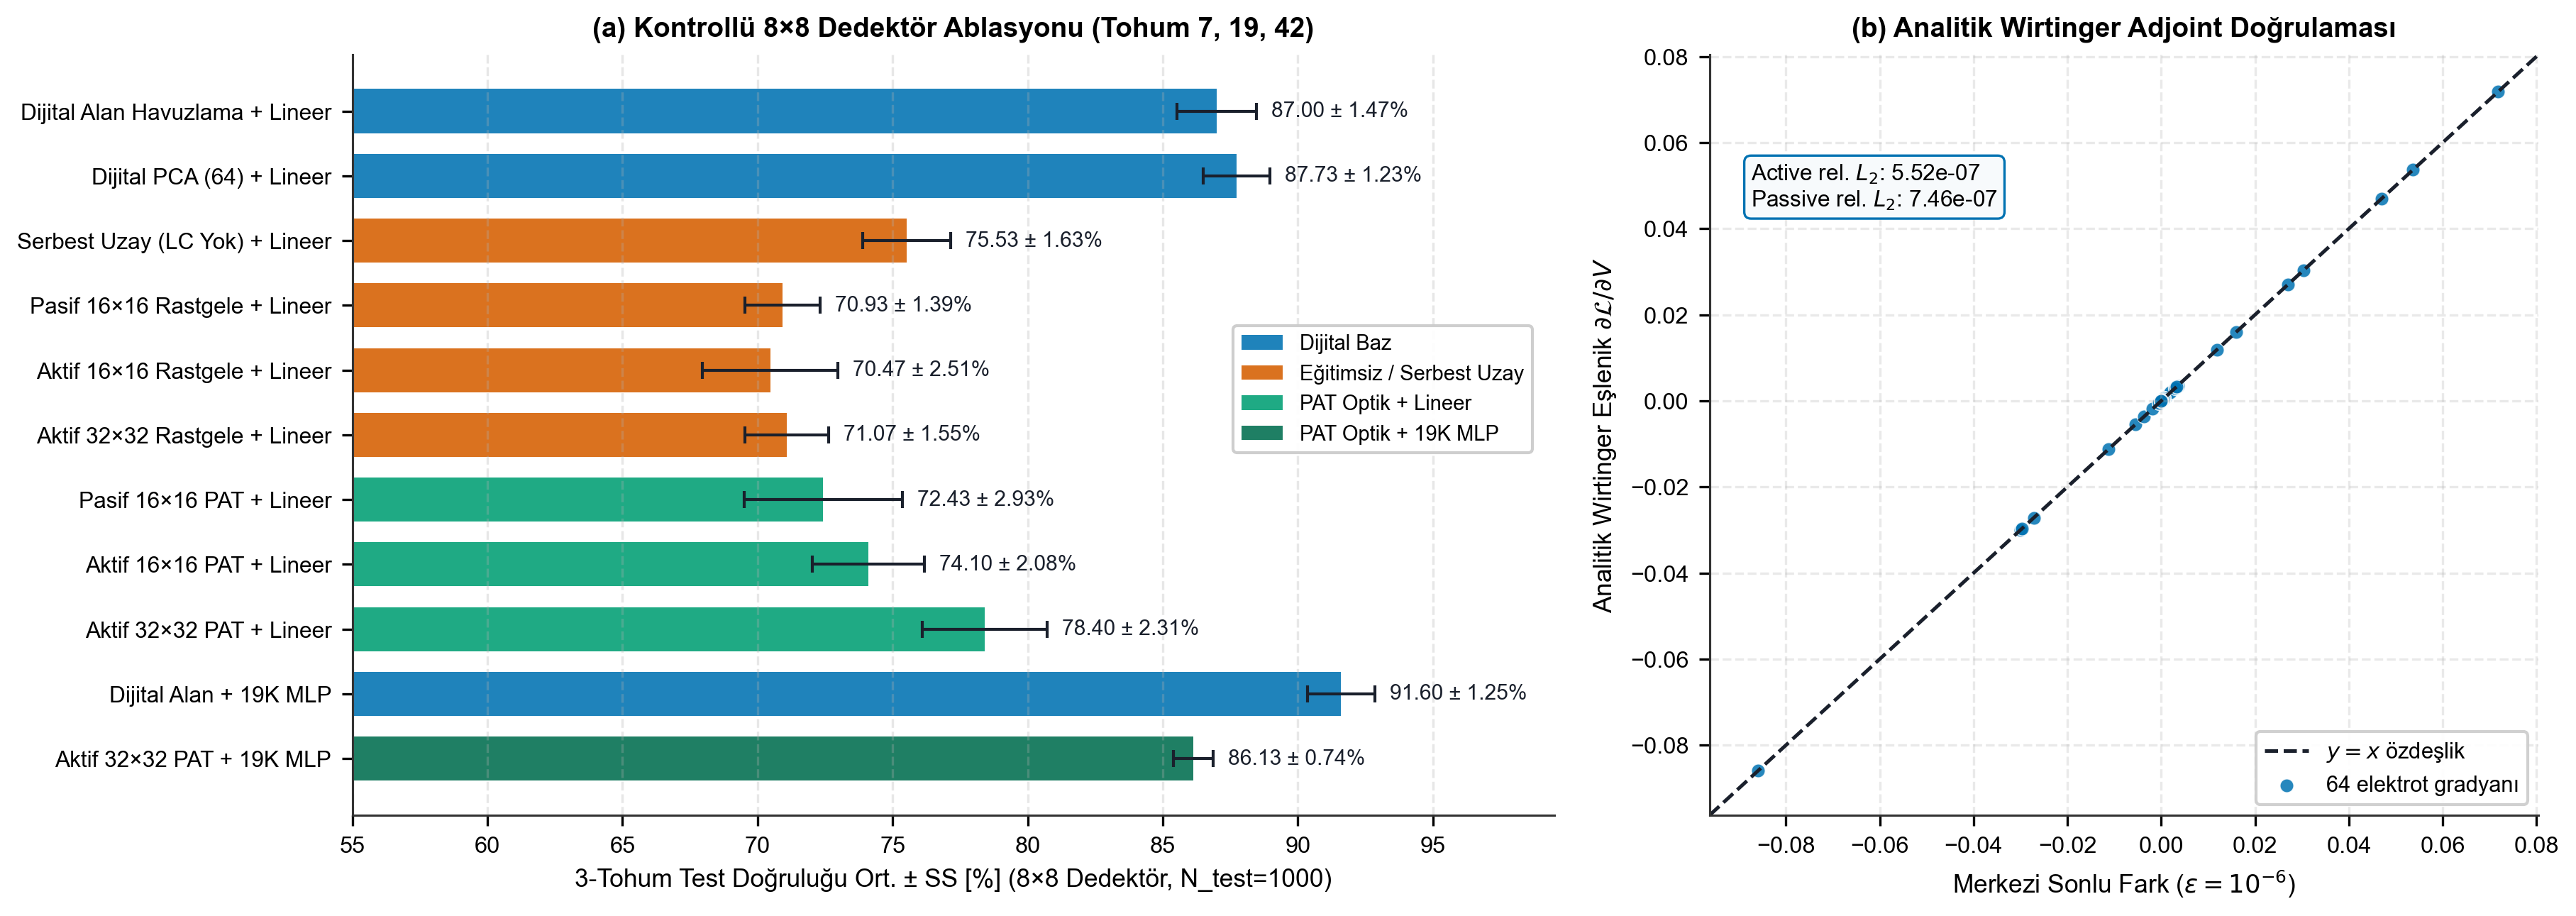
\includegraphics[width=0.98\textwidth]{figures/makale_fig3_ablasyon_pat_tr.png}
  \caption{\textbf{(a)}~Kusurlu fiziksel sistem sim\"ulat\"or\"unde $8\times 8$ dedekt\"or rejimindeki t\"um 11 e\c{s}le\c{s}mi\c{s} yap\i{}land\i{}rmada 3 tohumlu s\i{}z\i{}nt\i{}s\i{}z MNIST test do\u{g}ruluklar\i{} (ortalama $\pm$ 1~SS, $N_{\mathrm{test}}=1000$). PAT ile e\u{g}itilen $32\times 32$ aktif optik katman, e\c{s}le\c{s}mi\c{s} rastgele opti\u{g}i $+7{,}33$ puan ge\c{c}erken (\%78,40 ve \%71,07) do\u{g}rudan dijital alan havuzlaman\i{}n (\%87,00) 8,60 puan alt\i{}nda kal\i{}r. \textbf{(b)}~Analitik Wirtinger e\c{s}lenik gradyan\i{}n\i{}n merkezi sonlu farklarla ($\varepsilon=10^{-6}$) parametre bazl\i{} uyumu.}
  \label{fig:ablation_pat}
\end{figure*}

\subsection{Fizik-Fark\i{}ndal\i{}kl\i{} E\u{g}itim ve Karanl\i{}k-Kare Stabilizasyonu}
Ger\c{c}ek optik d\"uzeneklerde montaj kaymalar\i{}, s\i{}cakl\i{}k sapmalar\i{} ve okuma g\"ur\"ult\"us\"u bulunaca\u{g}\i{} i\c{c}in PAT d\"ong\"us\"u \cite{wright2022pat} ileri ge\c{c}i\c{s} \c{c}\i{}kt\i{}lar\i{}n\i{} kusurlu fiziksel sistem sim\"ulat\"or\"unden al\i{}rken, optik geri ad\i{}mlar\i{} \eqref{eq:wirtinger}--\eqref{eq:grad_v} ile nominal say\i{}sal ikiz \"uzerinden hesaplar (gradyans\i{}z yedek olarak SPSA \cite{spall1998spsa} tutulur). Ortam \i{}\c{s}\i{}\u{g}\i{} s\i{}z\i{}nt\i{}s\i{} alt\i{}nda s\i{}f\i{}r varyansa yak\i{}n kenar piksellerinin standartla\c{s}t\i{}rmada \c{s}i\c{s}mesini engellemek amac\i{}yla 16 kareli g\"ur\"ult\"ul\"u karanl\i{}k arka plan \c{c}\i{}karma ve yaln\i{}zca e\u{g}itim k\"umesine dayal\i{} bir standart sapma taban\i{} uygulan\i{}r:
\begin{equation}
  \tilde{\mathbf{f}} = \frac{(\mathbf{f}_{\mathrm{on}} - \mathbf{f}_{\mathrm{dark}}) - \bm{\mu}_{\mathrm{tr}}}{\max\!\left(\bm{\sigma}_{\mathrm{tr}},\, 0{,}05\cdot\operatorname{mean}(\bm{\sigma}_{\mathrm{tr}})\right)},
  \label{eq:sd_floor}
\end{equation}
burada $\bm{\mu}_{\mathrm{tr}}$ ve $\bm{\sigma}_{\mathrm{tr}}$ test s\i{}z\i{}nt\i{}s\i{} olmadan yaln\i{}zca e\u{g}itim verisinden hesaplan\i{}r.

\begin{table}[!t]
  \centering
  \caption{Sim\"ulasyon D\"uzene\u{g}i, Optik Geometri ve E\u{g}itim Hiperparametreleri}
  \label{tab:sim_setup}
  \begin{tabular}{@{}ll@{}}
    \toprule
    \textbf{Parametre} & \textbf{De\u{g}er / \c{S}artname} \\
    \midrule
    Dalga boyu $\lambda$ / Piksel ad\i{}m\i{} $\Delta x$ & $532\,\text{nm}$ / $47\,\mu\text{m}$ \\
    Eksenel mesafeler $Z_1$, $Z_2$ & $50\,\text{mm}$, $50\,\text{mm}$ ($10\,\text{cm}$ yol, $0{,}33\,\text{ns}$) \\
    Izgara boyutlar\i{} $N$ & $128\times 128$ ($6{,}02\,\text{mm}$), $256\times 256$ ($12{,}03\,\text{mm}$) \\
    ASM kritik boyut / Yay\i{}lma & $N_{\mathrm{crit}} = 12{,}0\,\text{px}$ / $0{,}283\,\text{mm}$ \\
    Koruma bantlar\i{} ($N=128$) & $1{,}69\,\text{mm}$ (giri\c{s}), $0{,}75\,\text{mm}$ (a\u{g}\i{}rl\i{}k) \\
    Aktif / Pasif kontrol s\i{}n\i{}rlar\i{} & $[1{,}05, 4{,}95]\,\text{V}$ ($4{,}64\,\text{rad}$) / $[-1, +1]$ ($0{,}921\,\text{rad}$) \\
    Eniyileyici & Adam ($\text{lr}_{\mathrm{opt}}=0{,}07\text{--}0{,}10$; $\text{lr}_{\mathrm{head}}=2{,}5\times 10^{-2}$ / $2{,}5\times 10^{-3}$) \\
    D\"uzenlileme / Takvim & $10^{-4}$ $L_2$; $16\text{--}22$ ep.\ (PAT), $40\text{--}45$ ep.\ (MLP); erken durdurma \\
    Kusurlu sistem hatalar\i{} & $47\,\mu\text{m}$ LCD/CMOS, $+1{,}2$/$-0{,}8\,\text{mm}$ $Z$, $29\,^\circ\text{C}$, \%2 drift \\
    Tohumlar / Test \"orne\u{g}i & $\{7, 19, 42\}$ / b\"olme ba\c{s}\i{}na $N_{\mathrm{test}}=1000$ \\
    \bottomrule
  \end{tabular}
\end{table}

% ============================================================================
\section{Say\i{}sal Bulgular ve Analiz}
% ============================================================================

\subsection{Kontroll\"u $8\times 8$ Dedekt\"or MNIST Ablasyonu}
T\"um say\i{}sal deneyler Python~3.11.9 / NumPy~2.2.3 ortam\i{}nda CPU \"uzerinde (Intel64 Family 6 Model 170) PAT yollar\i{}nda \texttt{complex64}, PAT-d\i{}\c{s}\i{}/de\u{g}erlendirme yollar\i{}nda \texttt{complex128} duyarl\i{}kla ve Tablo~\ref{tab:sim_setup}'de \"ozetlenen hiperparametrelerle \c{c}al\i{}\c{s}t\i{}r\i{}lm\i{}\c{s}t\i{}r. Elektronik okuma bant geni\c{s}li\u{g}i s\i{}k\i{} \c{s}ekilde k\i{}s\i{}tland\i{}\u{g}\i{}nda programlanabilir optik a\u{g}\i{}rl\i{}klar\i{}n net katk\i{}s\i{}n\i{} \"ol\c{c}mek i\c{c}in $8\times 8 = 64$ dedekt\"or \"uzerinde \"u\c{c} tohumla 11 e\c{s}le\c{s}mi\c{s} MNIST \cite{lecun1998mnist} yap\i{}land\i{}rmas\i{} kar\c{s}\i{}la\c{s}t\i{}r\i{}lm\i{}\c{s}t\i{}r ($N_{\mathrm{fit}}=2640$, $N_{\mathrm{val}}=360$, $N_{\mathrm{test}}=1000$). Fiziksel sim\"ulat\"or; vekil ikizin bilmedi\u{g}i $47\,\mu\text{m}$ LCD ve sens\"or kaymas\i{}, $+1{,}2\,\text{mm}/-0{,}8\,\text{mm}$ eksenel hata, $29\,^\circ\text{C}$ Haller s\i{}cakl\i{}k sapmas\i{} \cite{haller1975thermodynamic,li2005lc}, \%2 lazer drifti ve Gauss okuma g\"ur\"ult\"us\"u i\c{c}ermektedir (Tablo~\ref{tab:ablation}, \c{S}ekil~\ref{fig:ablation_pat}a).

\begin{table}[!t]
  \centering
  \caption{Kusurlu Sistemde Kontroll\"u MNIST Ablasyonu ($8\times 8$ Dedekt\"or, 3 Tohum, $N_{\mathrm{test}}=1000$)}
  \label{tab:ablation}
  \begin{tabular}{@{}llrrr@{}}
    \toprule
    \textbf{\#} & \textbf{Mimari / Yap\i{}land\i{}rma} & \textbf{Opt. W} & \textbf{Dij. W} & \textbf{Test (\%)} \\
    \midrule
    1 & Dijital Alan Havuzlama ($8\times 8$) + Lineer & 0 & 650 & $87{,}00 \pm 1{,}47$ \\
    2 & Dijital PCA Temeli ($64$-boyut) + Lineer & 0 & 650\rlap{\textsuperscript{a}} & $87{,}73 \pm 1{,}23$ \\
    3 & Yaln\i{}z Serbest Uzay K\i{}r\i{}n\i{}m\i{} (LC Yok) & 0 & 650 & $75{,}53 \pm 1{,}63$ \\
    4 & Pasif $16\times 16$ Rastgele + Lineer & 256 & 650 & $70{,}93 \pm 1{,}39$ \\
    5 & Aktif $16\times 16$ Rastgele + Lineer & 256 & 650 & $70{,}47 \pm 2{,}51$ \\
    6 & Aktif $32\times 32$ Rastgele + Lineer & 1.024 & 650 & $71{,}07 \pm 1{,}55$ \\
    7 & Pasif $16\times 16$ + PAT + Lineer & 256 & 650 & $72{,}43 \pm 2{,}93$ \\
    8 & Aktif $16\times 16$ + PAT + Lineer & 256 & 650 & $74{,}10 \pm 2{,}08$ \\
    \textbf{9} & \textbf{Aktif $32\times 32$ + PAT + Lineer} & \textbf{1.024} & \textbf{650} & \textbf{78,40 $\pm$ 2,31} \\
    10 & Dijital Alan Havuzlama ($8\times 8$) + MLP & 0 & 19.210 & $91{,}60 \pm 1{,}25$ \\
    \textbf{11} & \textbf{Aktif $32\times 32$ + PAT + MLP} & \textbf{1.024} & \textbf{19.210} & \textbf{86,13 $\pm$ 0,74} \\
    \bottomrule
  \end{tabular}
  \\[2pt]\footnotesize{\textsuperscript{a}E\u{g}itim k\"umesinden kurulan $784\times 64$ lineer PCA izd\"u\c{s}\"um matrisi hari\c{c}.}
\end{table}

Tablo~\ref{tab:ablation} iki net sonu\c{c} ortaya koymaktad\i{}r. Birincisi, optimize edilmemi\c{s} k\i{}r\i{}n\i{}m, uzamsal enerjiyi kaba pikseller aras\i{}nda da\u{g}\i{}tt\i{}\u{g}\i{} i\c{c}in do\u{g}rudan $8\times 8$ dijital g\"or\"unt\"ulemeye g\"ore do\u{g}rulu\u{g}u belirgin bi\c{c}imde d\"u\c{s}\"ur\"ur (\%70,47--\%71,07'ye kar\c{s}\i{} \%87,00). $32\times 32$ aktif LC a\u{g}\i{}rl\i{}klar\i{}n\i{}n PAT ile eniyilenmesi, e\c{s}le\c{s}mi\c{s} rastgele opti\u{g}e k\i{}yasla $+7{,}33$ puan (\%71,07 $\to$ \%78,40) ve yal\i{}n serbest uzaya k\i{}yasla $+2{,}87$ puan kazan\i{}m sa\u{g}lar. Buna kar\c{s}\i{}n $16\times 16$ optik \c{c}\"oz\"un\"url\"ukte pasif PAT (\%72,43 $\pm$ 2,93) ile aktif PAT (\%74,10 $\pm$ 2,08) bir standart sapma i\c{c}inde istatistiksel olarak e\c{s}de\u{g}erdir, \c{c}\"unk\"u dar $8\times 8$ okuma faz aral\i{}\u{g}\i{}ndan \c{c}ok okuma s\i{}ras\i{}n\i{} (rank) k\i{}s\i{}tlamaktad\i{}r. \.{I}kincisi, pozitif kare-yasa yo\u{g}unlu\u{g}u \"uzerinde \c{c}al\i{}\c{s}an tek bir programlanabilir k\i{}r\i{}n\i{}m katman\i{}, g\"ur\"ult\"us\"uz dijital $8\times 8$ alan havuzlaman\i{}n (\%78,40 ve \%87,00; 19K MLP ile \%86,13 ve \%91,60) gerisinde kal\i{}rken veri g\"ud\"uml\"u dijital PCA-64 izd\"u\c{s}\"um\"u do\u{g}rusal \"ust s\i{}n\i{}r\i{} \%87,73 $\pm$ 1,23 olarak belirler.

\subsection{MNIST ve Fashion-MNIST \"Uzerinde Tam $32\times 32$ Hibrit S\i{}n\i{}fland\i{}rma}
CMOS dedekt\"or \"org\"us\"un\"un $32\times 32$ (1.024 \"ozellik) boyutuna \c{c}\i{}kar\i{}lmas\i{}, hem MNIST \cite{lecun1998mnist} hem de 10 s\i{}n\i{}fl\i{} Fashion-MNIST \cite{xiao2017fashion} veri k\"umelerinde optik ve elektronik kapasitenin nas\i{}l etkile\c{s}ti\u{g}ini a\c{c}\i{}k\c{c}a g\"osterir (Tablo~\ref{tab:scaling}). $N_{\mathrm{train}}=6000$ iken, do\u{g}rulama k\"umesinde $\alpha$ se\c{c}imi yap\i{}lan d\"uzenlile\c{s}tirilmi\c{s} Ridge lineer okuyucuyla sabit rastgele $32\times 32$ optik maske MNIST'te ham $28\times 28$ piksellerle 1 standart sapma i\c{c}inde e\c{s}de\u{g}erdir (\%85,97 $\pm$ 2,05 ve \%85,43 $\pm$ 1,36); Fashion-MNIST'te ise PAT-e\u{g}itimli $32\times 32$ Ridge okuyucu ham piksellerin s\i{}n\i{}rda gerisindedir (\%79,80 $\pm$ 1,93 ve \%80,57 $\pm$ 0,95).

\begin{table}[!t]
  \centering
  \caption{Tam \"Ol\c{c}ekli $32\times 32$ Hibrit ve Dijital Kar\c{s}\i{}la\c{s}t\i{}rma (3 Tohum, $N_{\mathrm{test}}=1000$)}
  \label{tab:scaling}
  \begin{tabular}{@{}lrrrr@{}}
    \toprule
    \textbf{Yap\i{}land\i{}rma} & \textbf{Opt. W} & \textbf{Dij. W} & \textbf{MNIST (\%)} & \textbf{F-MNIST (\%)} \\
    \midrule
    Ham $28\times 28$ Dijital Ridge ($N=6\text{k}$) & 0 & 7.850 & $85{,}43 \pm 1{,}36$ & $80{,}57 \pm 0{,}95$ \\
    Opt. $16\times 16$, 256\"oz. Ridge ($N=2{,}5\text{k}$) & 256 & 2.570 & $81{,}90 \pm 1{,}08$ & --- \\
    Opt. $16\times 16$, 1024\"oz. Ridge ($N=2{,}5\text{k}$) & 256 & 10.250 & $84{,}13 \pm 1{,}22$ & --- \\
    Opt. $32\times 32$ Rast., 1024\"oz. Ridge ($N=6\text{k}$) & 1.024 & 10.250 & $85{,}97 \pm 2{,}05$ & --- \\
    Opt. $32\times 32$ PAT, 1024\"oz. Ridge ($N=6\text{k}$) & 1.024 & 10.250 & --- & $79{,}80 \pm 1{,}93$ \\
    \midrule
    Ham $28\times 28$ Dijital MLP ($N=6\text{k}$) & 0 & 203.530 & $93{,}93 \pm 0{,}99$ & $85{,}17 \pm 0{,}15$ \\
    $32\times 32$ Rastgele Optik + MLP & 1.024 & 264.970 & $94{,}20 \pm 0{,}95$ & $84{,}70 \pm 0{,}85$ \\
    $32\times 32$ PAT + MLP (Kusurlu) & 1.024 & 264.970 & $91{,}07 \pm 1{,}90$ & $81{,}47 \pm 1{,}27$ \\
    $32\times 32$ PAT + MLP (Nominal \.{I}kiz, \"ust s\i{}n\i{}r) & 1.024 & 264.970 & $94{,}67 \pm 0{,}55$ & $84{,}43 \pm 0{,}51$ \\
    \bottomrule
  \end{tabular}
\end{table}

Buna kar\c{s}\i{}l\i{}k $1024\to 256\to 10$ ReLU MLP (264.970 dijital a\u{g}\i{}rl\i{}k) eklendi\u{g}inde s\i{}n\i{}fland\i{}rma ba\c{s}ar\i{}m\i{}n\i{} elektronik kapasite belirler: nominal ikizde yeniden e\u{g}itilmi\c{s} PAT kafas\i{} (\%94,67 MNIST, \%84,43 Fashion-MNIST; donan\i{}m kalibrasyonu de\u{g}il, kusursuz vekil \"ust s\i{}n\i{}r\i{}), sabit rastgele optikli MLP (\%94,20 ve \%84,70) ve ham piksel MLP (\%93,93 ve \%85,17) yakla\c{s}\i{}k $0{,}5$ puan i\c{c}inde toplanmaktad\i{}r; telafi edilmemi\c{s} kusurlu sistemde ise PAT MLP \%91,07 (MNIST) ve \%81,47 (Fashion-MNIST) elde etmektedir. K\i{}s\i{}tl\i{} $8\times 8$ Fashion-MNIST rejiminde ise (\c{S}ekil~\ref{fig:realism}c) PAT lineer s\i{}n\i{}fland\i{}rma e\c{s}le\c{s}mi\c{s} rastgele opti\u{g}i $+4{,}76$ puan a\c{s}arak \%71,63'e (\%66,87'ye kar\c{s}\i{}), 19K MLP ile \%77,50'e ula\c{s}makta; do\u{g}rudan $8\times 8$ dijital havuzlama \%77,93 (lineer) ve \%81,43 (MLP) vermektedir (yani optik katman lineer okumada dijital taban\i{}n bile gerisindedir).

\begin{figure*}[!t]
  \centering
  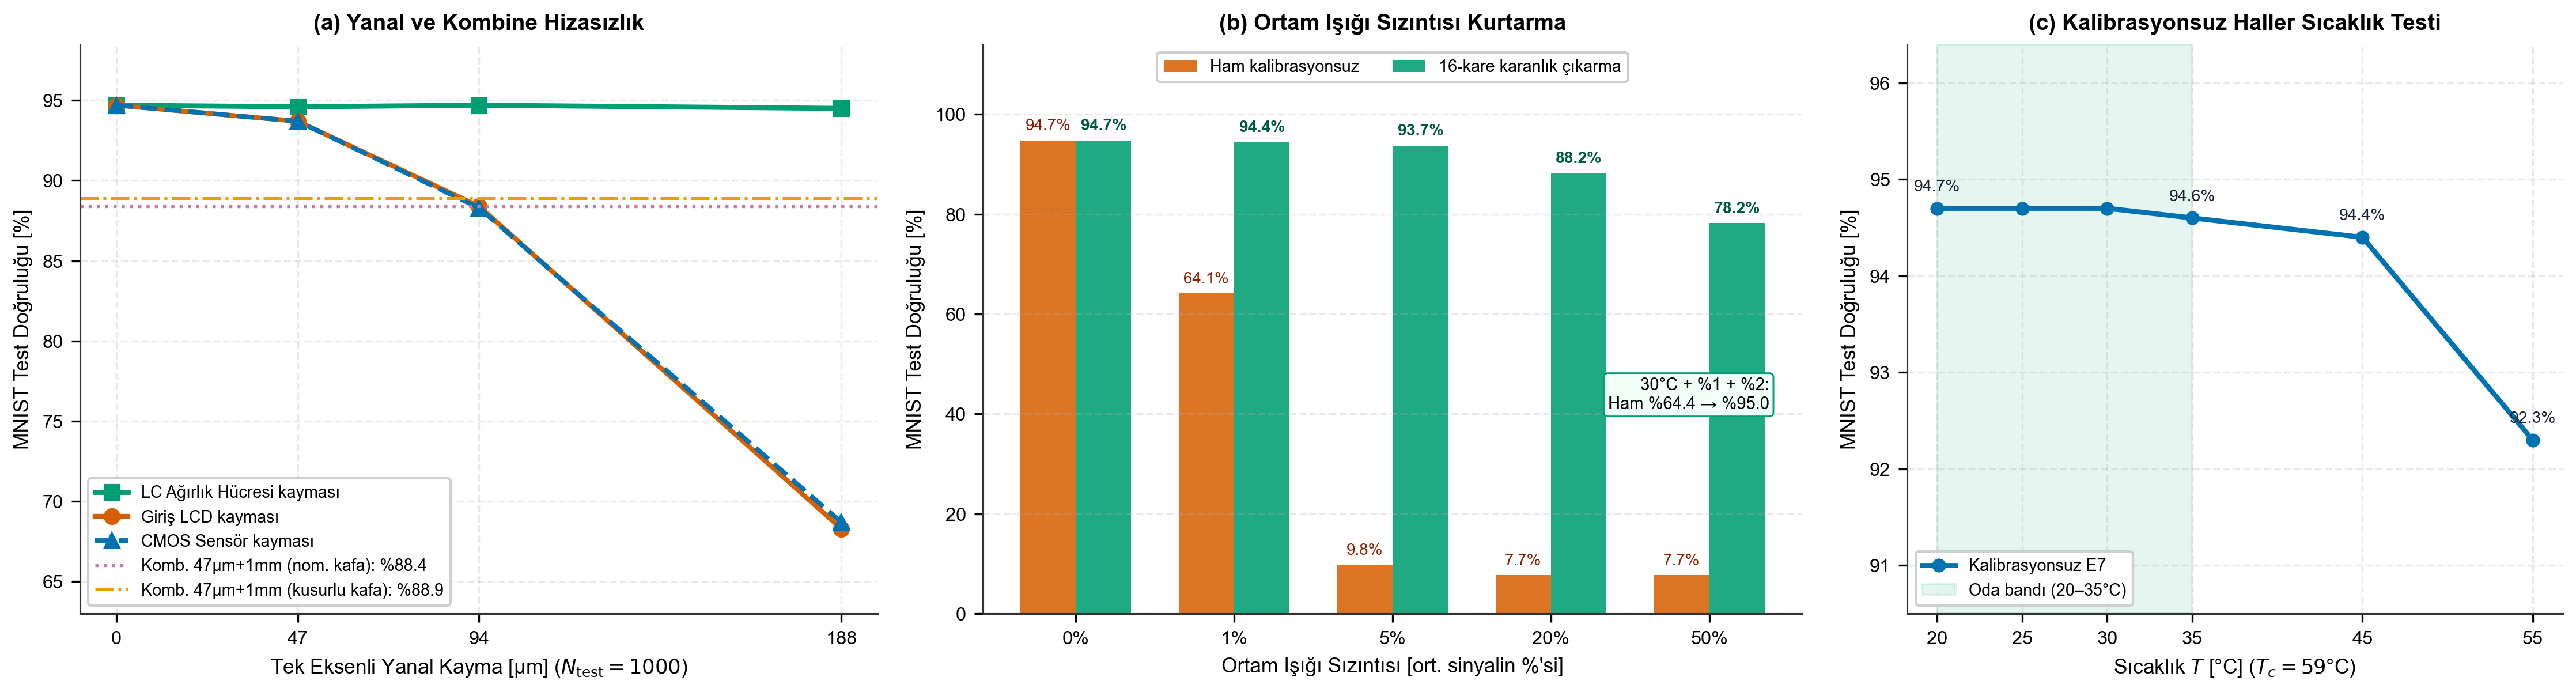
\includegraphics[width=0.96\textwidth]{figures/makale_fig4_dayanim_tr.png}
  \caption{Mekanik ve \c{c}evresel dayan\i{}kl\i{}l\i{}k testleri ($N_{\mathrm{test}}=1000$, tohum~7, nominal baz \%94,7): \textbf{(a)}~LC a\u{g}\i{}rl\i{}k h\"ucresi ($188\,\mu\text{m}$'de $\%94{,}7 \to \%94{,}5$), giri\c{s} LCD (\%94,7 $\to$ \%68,3) ve CMOS sens\"or (\%94,7 $\to$ \%68,7) tek eksenli yanal kaymalar\i{} ile kombine $47\,\mu\text{m} + 1\,\text{mm}$ sapmas\i{} (nominal kafa \%88,4; kusurla e\u{g}itilmi\c{s} kafa \%88,9, baz \%89,0); \textbf{(b)}~ortam \i{}\c{s}\i{}\u{g}\i{} s\i{}z\i{}nt\i{}s\i{}nda ham \c{c}\"ok\"u\c{s}e kar\c{s}\i{} 16 kareli karanl\i{}k-kare \c{c}\i{}karma ve $30\,^\circ\text{C}+\%1+\%2$ birle\c{s}ik iyile\c{s}me (\%64,4 $\to$ \%95,0); \textbf{(c)}~kalibrasyonsuz E7 Haller s\i{}cakl\i{}k taramas\i{} ($20\text{--}55\,^\circ\text{C}$, $T_c=59\,^\circ\text{C}$).}
  \label{fig:robustness}
\end{figure*}

\subsection{Mekanik Hizalama, S\i{}cakl\i{}k Kaymas\i{} ve Ortam I\c{s}\i{}\u{g}\i{} Dayan\i{}m\i{}}
Harici referans kolu i\c{c}ermeyen ortak-yol optik d\"uzlemde eksenel yo\u{g}unluk tolerans\i{} Talbot uzunlu\u{g}uyla ($z_T = 2\Delta x^2/\lambda \approx 8{,}3\,\text{mm}$) belirlenir. $1.000$ MNIST test \"orne\u{g}inde (tohum~7, baz \%94,7, \c{S}ekil~\ref{fig:robustness}a), LC a\u{g}\i{}rl\i{}k katman\i{}n\i{}n $188\,\mu\text{m}$ yanal kaymas\i{} yaln\i{}zca $0{,}2$ puan kay\i{}p olu\c{s}turur (\%94,7 $\to$ \%94,5) \c{c}\"unk\"u gelen alan uzamsal olarak yumu\c{s}akt\i{}r. Giri\c{s} LCD ve CMOS sens\"or kaymalar\i{} $47\,\mu\text{m}$ (\%93,7) \"otesinde daha keskin d\"u\c{s}\"er ($188\,\mu\text{m}$'de \%68,3 ve \%68,7); eksenel $\Delta Z_1 \in [0, 8\,\text{mm}]$ sapmalar\i{} ise \%94,3--\%94,7 aral\i{}\u{g}\i{}nda kal\i{}r. T\"um d\"uzlemlerin e\c{s}zamanl\i{} $47\,\mu\text{m}$ yanal ve $+1\,\text{mm}$ eksenel kayd\i{}\u{g}\i{} kombine testte nominal kafa \%88,4'e ($-6{,}3$ puan) inerken, pert\"urbe sistemle e\u{g}itilmi\c{s} kafa \%89,0 baz\i{}na g\"ore \%88,9 de\u{g}erini korur ($-0{,}1$ puan).

Haller ba\u{g}\i{}nt\i{}s\i{}yla \cite{haller1975thermodynamic,li2005lc} modellenen termal kaymada:
\begin{equation}
  \frac{\Delta n(T)}{\Delta n(25\,^\circ\text{C})} = \left(\frac{T_c - T}{T_c - 25}\right)^{\!\beta}, \quad T_c = 59\,^\circ\text{C},\; \beta = 0{,}22,
  \label{eq:haller}
\end{equation}
kalibrasyonsuz do\u{g}ruluk $20\text{--}45\,^\circ\text{C}$ aras\i{}nda \%94,4--\%94,7 d\"uzeyinde kal\i{}p berrakla\c{s}ma noktas\i{}na yak\i{}n $55\,^\circ\text{C}$'de \%92,3'e iner (\c{S}ekil~\ref{fig:robustness}c). Arka plan \c{c}\i{}karma olmadan ortalama sinyalin \%1 ve \%5'i kadar ortam \i{}\c{s}\i{}\u{g}\i{} s\i{}z\i{}nt\i{}s\i{} do\u{g}rulu\u{g}u \%64,1 ve \%9,8'e d\"u\c{s}\"ur\"urken, 16 kareli karanl\i{}k arka plan \c{c}\i{}karma ve \eqref{eq:sd_floor} s\i{}ras\i{}yla \%94,4 (\%1), \%93,7 (\%5), \%88,2 (\%20) ve \%78,2 (\%50) sa\u{g}lar; kombine $30\,^\circ\text{C}$ + \%1 s\i{}z\i{}nt\i{} + \%2 lazer drift testini ise \%64,4'ten \%95,0'a \c{c}\i{}kar\i{}r. Lazer g\"uc\"u $\pm 10\%$ de\u{g}i\c{s}ti\u{g}inde do\u{g}ruluk \%94,2--\%94,9 aral\i{}\u{g}\i{}ndad\i{}r.

\begin{figure*}[!t]
  \centering
  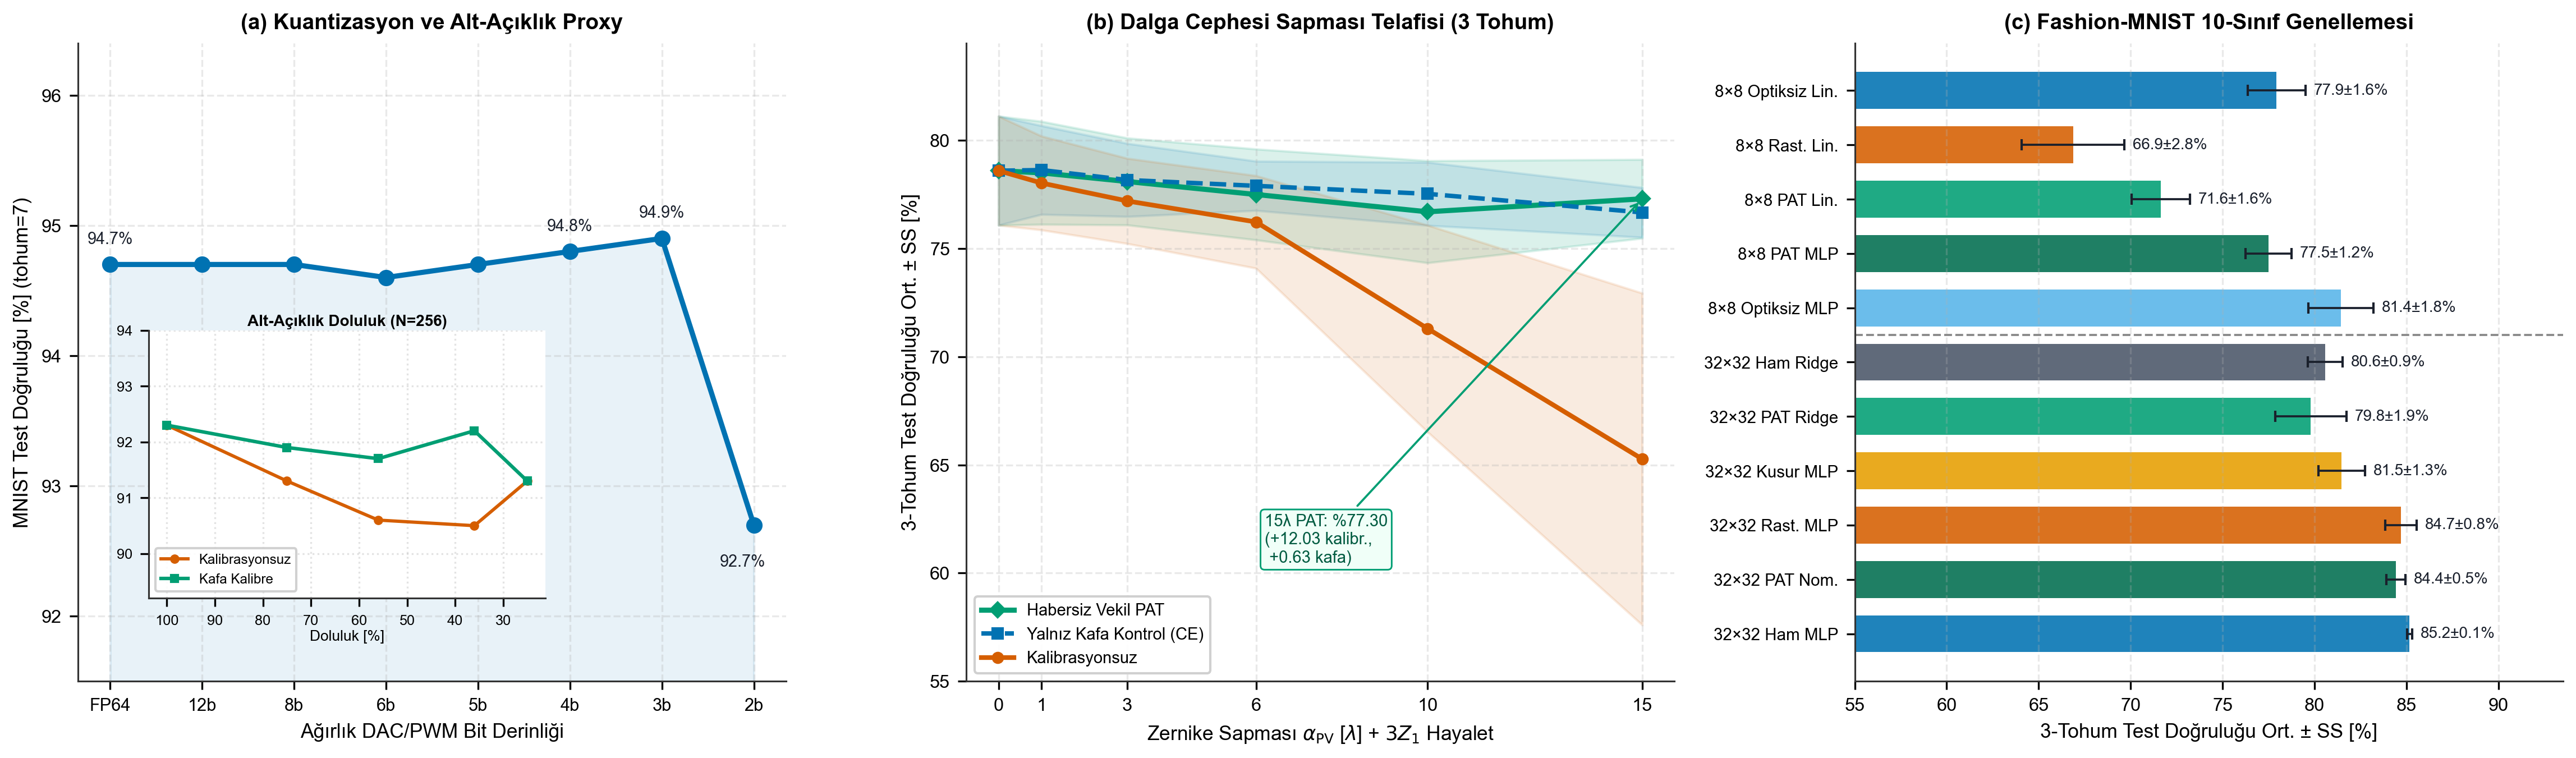
\includegraphics[width=0.98\textwidth]{figures/makale_fig5_gercekcilik_tr.png}
  \caption{Donan\i{}m ger\c{c}ek\c{c}ili\u{g}i ve genelleme testleri ($N_{\mathrm{test}}=1000$): \textbf{(a)}~8-bit HDMI giri\c{s} ve $b$-bit a\u{g}\i{}rl\i{}k basamaklamas\i{} (4-bit'e kadar \%94,6--\%94,9, 2-bit'te \%92,7) ve makro-piksel alt-a\c{c}\i{}kl\i{}k dolulu\u{g}u i\c{c} grafi\u{g}i (\%25 dolulukta kalibrasyonsuz $\%92{,}3 \to \%91{,}3$, kafa kalibre $\%92{,}3 \to \%91{,}3$); \textbf{(b)}~3 tohumlu Zernike dalga cephesi sapmalar\i{} ($0\text{--}15\lambda$ PV + $3Z_1$ hayalet): kalibrasyonsuz (\%65,27 $\pm$ 7,67), e\c{s}le\c{s}mi\c{s} CE yaln\i{}z-kafa kontrol\"u (\%76,67 $\pm$ 1,15) ve habersiz vekil PAT (\%77,30 $\pm$ 1,82); \textbf{(c)}~3 tohumlu 10 s\i{}n\i{}fl\i{} Fashion-MNIST kar\c{s}\i{}la\c{s}t\i{}rmas\i{}.}
  \label{fig:realism}
\end{figure*}

\subsection{Bit Kuantizasyonu, Alt-A\c{c}\i{}kl\i{}k Vekili ve Dalga Cephesi Sapmas\i{}}
Masa\"ust\"u kurulumu \"oncesi \"u\c{c} ek ger\c{c}ek\c{c}ilik testi daha y\"ur\"ut\"ulm\"u\c{s}t\"ur (\c{S}ekil~\ref{fig:realism}a--b). 8-bit HDMI giri\c{s} ve $b$-bit LC kontrol gerilimi kuantizasyonunda (tohum~7) do\u{g}ruluk 4-bit'e (16 gerilim seviyesi) kadar \%94,6--\%94,9'da kal\i{}p 2-bit'te \%92,7 olmaktad\i{}r. $N=256$ \i{}zgarada \%100'den \%25'e inen makro-piksel alt-a\c{c}\i{}kl\i{}k vekil testinde kalibrasyonsuz do\u{g}ruluk \%92,3'ten \%91,3'e inerken, dijital kafa yeniden kalibrasyonu ayn\i{} aral\i{}kta \%91,3 vermektedir.

Be\c{s}inci derece Zernike sapmalar\i{} ($0\text{--}15\lambda$ PV) ile $3Z_1$ Fabry--P\'erot hayaleti ($0{,}04$ genlik) eklendi\u{g}inde, t\"um ko\c{s}ullar e\c{s}it \c{c}apraz entropi Adam kafas\i{}yla de\u{g}erlendirildi\u{g}inde dikkate de\u{g}er bir ayr\i{}m g\"or\"ul\"ur (\c{S}ekil~\ref{fig:realism}b): $1\lambda$--$10\lambda$ aral\i{}\u{g}\i{}nda donmu\c{s} optikle yaln\i{}z kafay\i{} yeniden kalibre etmek kayb\i{}n neredeyse tamam\i{}n\i{} telafi ederek (\%78,63 ve \%77,53) habersiz vekil PAT'ye (\%78,50 ve \%76,70) denk sonu\c{c} verirken, a\u{g}\i{}r $15\lambda$ sapmada kalibrasyonsuz sistem \%65,27 $\pm$ 7,67'ye d\"u\c{s}mekte, yaln\i{}z-kafa kalibrasyonu \%76,67 $\pm$ 1,15'e, ortak optik adaptasyonlu PAT ise \%77,30 $\pm$ 1,82'ye ula\c{s}maktad\i{}r (bu $+0{,}63$ puanl\i{}k fark birle\c{s}ik standart sapman\i{}n i\c{c}inde kald\i{}\u{g}\i{}ndan \"ust\"unl\"uk de\u{g}il, yaln\i{}zca marjinal bir e\u{g}ilim olarak okunmal\i{}d\i{}r).

Ayr\i{}ca parametrik pert\"urbasyon d\"uzeni\u{g}inin ifade edemedi\u{g}i daha sert bir rejim de s\i{}nanm\i{}\c{s}t\i{}r: fiziksel ileri modelin $\pm\%10$ pert\"urbe LC aktar\i{}m e\u{g}risi, $0{,}90$ kamera gammas\i{} ve \c{c}arp\i{}msal benek ta\c{s}\i{}d\i{}\u{g}\i{} (vekilin fizi\u{g}inde hi\c{c}biri bulunmayan) \emph{yap\i{}sal model-uyumsuzlu\u{g}u} ko\c{s}ulu. Ayn\i{} $8\times 8$ MNIST protokol\"unde kalibrasyonsuz ideal a\u{g}\i{}rl\i{}klar \%71,30 $\pm$ 1,08, e\c{s}le\c{s}mi\c{s} yaln\i{}z-kafa kalibrasyonu \%79,13 $\pm$ 2,39 ve habersiz vekil PAT \%76,80 $\pm$ 1,65 vermektedir: PAT kalibrasyonsuz kayb\i{}n \c{c}o\u{g}unu telafi etse de \c{s}a\c{s}\i{}rt\i{}c\i{} bi\c{c}imde \emph{yaln\i{}z-kafa kalibrasyonunun gerisinde} kalmaktad\i{}r. Bu, uyumsuzluk parametrikten yap\i{}sala ge\c{c}ti\u{g}inde dijital \"ozellik normalizasyonunun, hatal\i{} bir vekil \"uzerinden hesaplanan optik a\u{g}\i{}rl\i{}k g\"uncellemelerinden daha etkili telafi sa\u{g}layabildi\u{g}ini g\"ostermektedir.

\begin{table}[!t]
  \centering
  \caption{Tahmini Prototip Malzeme B\"ut\c{c}esi (BOM)}
  \label{tab:bom}
  \begin{tabular}{@{}llr@{}}
    \toprule
    \textbf{Alt Sistem} & \textbf{Se\c{c}ilen Donan\i{}m} & \textbf{Tutar (USD)} \\
    \midrule
    Optik Giri\c{s} & $532\,\text{nm}$ DPSS ($100\,\text{mW}$) + Geni\c{s}letici + mSLA LCD & 150 \\
    Aktif A\u{g}\i{}rl\i{}klar & 2. mSLA TFT-LCD (veya ITO H\"ucre + AC-PWM) & 90--230 \\
    Okuma ve Kontrol & RPi Camera 3 (IMX708, $12\,\text{MP}$) + M12 + RPi 5 & 125 \\
    Optomekanik & Optik Ray, Tutucular, Karart\i{}lm\i{}\c{s} Kutu, Filtre & 262 \\
    \midrule
    Ara Toplam & Temel optik ve elektronik bile\c{s}enler & 627--767 \\
    \textbf{Toplam (+\%25)} & \textbf{Yedek pay\i{} dahil masa\"ust\"u prototip} & \textbf{784--959} \\
    \bottomrule
  \end{tabular}
\end{table}

% ============================================================================
\section{Tart\i{}\c{s}ma, S\i{}n\i{}rl\i{}l\i{}klar ve Donan\i{}m Yol Haritas\i{}}
% ============================================================================

Tablo~\ref{tab:bom}'te kalemlendirilen mod\"uler optik ray kurulumu do\u{g}rudan bile\c{s}enlerde 627--767~USD, \%25 yedek pay\i{}yla 784--959~USD tutmaktad\i{}r. Sistemde \"u\c{c} farkl\i{} zaman \"ol\c{c}e\u{g}i birbirinden ayr\i{} tutulmal\i{}d\i{}r: $10\,\text{cm}$ optik yol boyunca koherent foton ge\c{c}i\c{s}i $\sim 0{,}33\,\text{ns}$ s\"urerken, ger\c{c}ek donan\i{}m ak\i{}\c{s} h\i{}z\i{}n\i{} $60\,\text{Hz}$ LCD/kamera \c{c}er\c{c}eve d\"ong\"us\"u ($\sim 16{,}7\,\text{ms}$) ve a\u{g}\i{}rl\i{}k g\"uncellemelerinde $\sim 50\,\text{ms}$ nematik gev\c{s}eme s\"uresi belirler; $N=128^2$ \i{}zgarada CPU \"uzerindeki derlenmemi\c{s} NumPy ASM sim\"ulasyonu ise 50 \c{c}al\i{}\c{s}mada $1{,}04\,\text{ms}$ ortanca s\"urede (Intel64 Family 6 Model 170 CPU, Python~3.11.9 / NumPy~2.2.3, ortalama $1{,}27\,\text{ms}$, IQR $0{,}63\,\text{ms}$, aral\i{}k $0{,}84\text{--}2{,}23\,\text{ms}$) tamamlanmaktad\i{}r.

Fiziksel montaj basitle\c{s}tirilmi\c{s} 2B modellerde yer almayan \"u\c{c} m\"uhendislik ko\c{s}ulu gerektirir: RPi Camera Module~3'\"un IMX708 sens\"or\"u ($6{,}45 \times 3{,}63\,\text{mm}$) k\i{}sa eksende $4{,}51\text{--}6{,}02\,\text{mm}$ k\i{}r\i{}n\i{}m alan\i{}ndan dar oldu\u{g}undan $\sim 1{,}6\times$ k\"u\c{c}\"ult\"uc\"u M12 r\"ole opti\u{g}i gerekir; $100\,\text{mW}$ $532\,\text{nm}$ DPSS lazer S\i{}n\i{}f~3B olmas\i{} nedeniyle OD~4+ g\"ozl\"uk, \i{}\c{s}\i{}k s\i{}zd\i{}rmaz kasa ve $808/1064\,\text{nm}$ pompa ka\c{c}a\u{g}\i{}n\i{} kesen IR filtre gerektirir; ayr\i{}ca PCA9685 PWM kartlar\i{} tek kutuplu darbe \"uretti\u{g}inden \c{c}\i{}plak ITO elektrotlarda elektrolizi \"onlemek i\c{c}in AC polarite-evirici s\"ur\"uc\"u devre olmadan kullan\i{}lmamal\i{}d\i{}r.

\subsection{S\i{}n\i{}rl\i{}l\i{}klar}
Sekiz temel s\i{}n\i{}rl\i{}l\i{}k bu say\i{}sal bulgular\i{}n kapsam\i{}n\i{} belirlemektedir. \.{I}lk olarak t\"um do\u{g}ruluk ve dayan\i{}kl\i{}l\i{}k verileri dalga-opti\u{g}i sim\"ulasyonlar\i{}na dayanmaktad\i{}r; fiziksel kurulum, hizalama ve ger\c{c}ek sens\"or g\"ur\"ult\"us\"u \"ol\c{c}\"umleri sonraki deneysel a\c{s}amay\i{} olu\c{s}turmaktad\i{}r. \.{I}kinci olarak $8\times 8$ dedekt\"orlerde, okuma kafas\i{} ve e\u{g}itim protokol\"u birebir e\c{s}lendi\u{g}inde PAT optik katman\i{} e\c{s}le\c{s}mi\c{s} rastgele opti\u{g}i $+7{,}33$ puan ge\c{s}se de do\u{g}rudan dijital alan havuzlaman\i{}n $8{,}60$ puan gerisinde kalmaktad\i{}r; $32\times 32$'de 265K parametreli MLP eklendi\u{g}inde ise s\i{}n\i{}fland\i{}rmay\i{} elektronik kafa bask\i{}layarak farklar\i{} $\sim 0{,}5$ puan i\c{c}ine s\i{}k\i{}\c{s}t\i{}rmaktad\i{}r.

\"U\c{c}\"unc\"u s\i{}n\i{}rl\i{}l\i{}k Denklem~\eqref{eq:jones}'n\i{}n paralel ECB h\"ucresini modellemesidir; ticari TN mSLA panellerdeki polarizasyon d\"on\"u\c{s}\"u \cite{lu1990lctv} deneysel lookup tablosu gerektirir. D\"ord\"unc\"us\"u, skaler sim\"ulasyonlar monokrom d\"uzlem dalga varsaymakta; DPSS lazer benek g\"ur\"ult\"us\"u, sonlu koherens uzunlu\u{g}u ve $0{,}04$ hayalet d\i{}\c{s}\i{}ndaki \c{c}oklu yans\i{}malar\i{} ihmal etmektedir. Be\c{s}incisi, her $32\times 32$ a\u{g}\i{}rl\i{}k blo\u{g}u onlarca $47\,\mu\text{m}$ mSLA alt-pikselini gruplad\i{}\u{g}\i{}ndan $N=256$ alt-a\c{c}\i{}kl\i{}k testi \"ol\c{c}eklenmi\c{s} bir vekil niteli\u{g}indedir. Alt\i{}nc\i{}s\i{}, varsay\i{}lan kusurlu sistem sim\"ulat\"or\"u vekille ayn\i{} skaler ASM fizik s\i{}n\i{}f\i{}n\i{} payla\c{s}t\i{}\u{g}\i{}ndan parametrik pert\"urbasyonu (kayma, s\i{}cakl\i{}k, drift, g\"ur\"ult\"u) s\i{}nar, yap\i{}sal model hatas\i{}n\i{} s\i{}namaz; bu nedenle pert\"urbe LC e\u{g}risi, kamera gammas\i{} ve \c{c}arp\i{}msal benek i\c{c}eren yap\i{}sal-uyumsuzluk varyant\i{} eklenmi\c{s} ve PAT'\i{}n bu daha zorlu rejimdeki davran\i{}\c{s}\i{} B\"ol\"um~IV'te raporlanm\i{}\c{s}t\i{}r. Yedincisi, ger\c{c}ek donan\i{}mda her PAT ileri ge\c{c}i\c{s}i bir LCD/kamera edinim d\"ong\"us\"u gerektirir (60~Hz'de \"ornek ba\c{s}\i{}na $\sim 16{,}7\,\text{ms}$); binlerce g\"or\"unt\"ul\"uk bir epok sim\"ulasyondaki milisaniyeler yerine dakikalar--saatler s\"urer, dolay\i{}s\i{}yla buradaki PAT kazan\i{}mlar\i{} pratik \c{c}evrimi\c{c}i e\u{g}itim h\i{}z\i{}n\i{} de\u{g}il yaln\i{}zca fizibiliteyi g\"osterir. Son olarak t\"um \c{c}oklu-tohum k\i{}yaslar\i{} yaln\i{}z \"u\c{c} tohum ve sabit e\u{g}itim/test alt k\"umeleriyle yap\i{}lm\i{}\c{s}t\i{}r ve tek bir kusurlu d\"uzenek i\c{c}in e\u{g}itilen a\u{g}\i{}rl\i{}klar, Keskinlik-Fark\i{}ndal\i{}kl\i{} E\u{g}itim \cite{sat2026pnn} gibi y\"ontemlerle geni\c{s}letilmedik\c{c}e farkl\i{} hizalanm\i{}\c{s} ikinci bir h\"ucreye do\u{g}rudan aktar\i{}lamaz.

% ============================================================================
\section{Sonu\c{c}}
% ============================================================================

Nematik Rayleigh--Gans sa\c{c}\i{}lma s\i{}n\i{}rlar\i{} (15--40~dB/cm) ve Alt--Pleshko RMS voltaj k\i{}s\i{}tlar\i{} ($5{,}28\times$ daralma) temelinde sentezlenen ortak-yol ZERRE (Model H) mimarisi, ticari mSLA ekranlar\i{} 784--959~USD b\"ut\c{c}e s\i{}n\i{}r\i{} i\c{c}inde bir araya getirmektedir. Skaler ASM k\i{}r\i{}n\i{}m\i{} \"uzerinden t\"uretilen Wirtinger e\c{s}lenik operat\"or\"u, kusurlu sim\"ulasyonlarda PAT e\u{g}itimini m\"umk\"un k\i{}larak $8\times 8$ lineer MNIST do\u{g}rulu\u{g}unu e\c{s}le\c{s}mi\c{s} rastgele opti\u{g}e g\"ore $+7{,}33$ puan art\i{}rm\i{}\c{s} (\%78,40), ancak do\u{g}rudan dijital alan havuzlaman\i{}n \%87,00'sinin $8{,}60$ puan gerisinde kalm\i{}\c{s}t\i{}r. $32\times 32$ hibrit okumada nominal ikiz \"ust s\i{}n\i{}r\i{} MNIST'te \%94,67 ve Fashion-MNIST'te \%84,43'e ula\c{s}\i{}rken kusurlu sistemde \%91,07 ve \%81,47 elde edilmi\c{s}; rastgele optik + MLP'nin \%94,20 ile e\c{s}de\u{g}er olmas\i{} optik katman\i{}n hesaplama katk\i{}s\i{}n\i{}n \"ol\c{c}\"ulebilir olmad\i{}\u{g}\i{}n\i{}, \c{c}al\i{}\c{s}man\i{}n mimari s\i{}n\i{}rlar\i{} ve deneysel kurulum ad\i{}mlar\i{}n\i{} a\c{c}\i{}k\c{c}a ortaya koyan bir fizibilite de\u{g}erlendirmesi sundu\u{g}unu g\"ostermi\c{s}tir.

% ============================================================================
\section*{Veri ve Kod Eri\c{s}ilebilirli\u{g}i}
% ============================================================================
T\"um Python dalga-opti\u{g}i sim\"ulasyon kodlar\i{} (\texttt{zerre\_twin.py}, \texttt{zerre\_pat\_torch.py}), etkile\c{s}imli WebGL/ASM g\"orselle\c{s}tiricisi (\texttt{start\_server.py}), otomatik fizik birim testleri (\texttt{tests/test\_zerre\_physics.py}), 3 tohumlu k\i{}yaslama \c{c}\i{}kt\i{}lar\i{} (\texttt{makale/scripts/paper\_results.json}) ve \c{s}ekil/makale derleme betikleri; yaz\i{}l\i{}m kodlar\i{} i\c{c}in \textbf{MIT Lisans\i{}}, makale metni ve \c{s}ekiller i\c{c}in ise \textbf{CC BY 4.0 Lisans\i{}} alt\i{}nda standart MNIST ve Fashion-MNIST yerel \"onbellek deste\u{g}iyle \url{https://github.com/hamzasolak/zerre} adresinde (s\"ur\"um etiketi \texttt{v0.5.0}; Yazar ORCID: \url{https://orcid.org/0009-0004-7541-9620}) yay\i{}mlanmaktad\i{}r.

\section*{Finansman}
Bu \c{c}al\i{}\c{s}ma herhangi bir kurum veya ticari fon deste\u{g}i olmaks\i{}z\i{}n ba\u{g}\i{}ms\i{}z ara\c{s}t\i{}rma olarak y\"ur\"ut\"ulm\"u\c{s}t\"ur.

\section*{{\c{C}}\i{}kar {\c{C}}at\i{}\c{s}mas\i{} Beyan\i{}}
Yazar herhangi bir \c{c}\i{}kar \c{c}at\i{}\c{s}mas\i{} bulunmad\i{}\u{g}\i{}n\i{} beyan eder.

\section*{Te\c{s}ekk\"ur}
Makalenin I--VI. B\"ol\"umlerinde \"uslup d\"uzenleme, LaTeX bi\c{c}imlendirme ve kod-do\u{g}rulama denetimi i\c{c}in \"uretken yapay zek\^a ara\c{c}lar\i{}ndan (Gemini ve Claude) yararlan\i{}lm\i{}\c{s}t\i{}r; fiziksel tasar\i{}m, dalga-opti\u{g}i sim\"ulasyon kodlar\i{}, \c{c}ok-tohumlu deneylerin y\"ur\"ut\"ulmesi ve t\"um bilimsel iddialar ile sonu\c{c}lar tamamen yazar\i{}n sorumlulu\u{g}undad\i{}r.

\balance
\bibliographystyle{IEEEtran}
\bibliography{references}

\end{document}
